\chapter{Потоковые кубиты в волноводе: изготовление и характеризация}

В этой главе излагаются результаты измерений одиночных сверхпроводниковых потоковых кубитов, сильно связанных с волноводом --- микроволновой копланарной проходной линией на чипе. Для проведения экспериментов по нелинейному рассеянию света требовалось изготовить <<искусственный атом>> --- двухуровневую систему, сильно связанную с внешним микроволновым излучением, свободно распространяющимся в пространстве. Описывается подход к проектированию образцов, в частности, подбору параметров, которые позволяют достичь режима сильной связи. Описывается процесс изготовления образцов с использованием методов электронной и лазерной литографии. Затем излагаются экспериментальные условия, необходимые для изучения квантовой динамики такого кубита, а также процесс сборки измерительной схемы внутри криостата растворения. Приводятся результаты измерений коэффициента отражения резонансного микроволнового сигнала, а также результаты измерения спектра неэластичного рассеяния и излучение при эволюции кубита под действием внешнего поля. При помощи теоретической модели, подгоняемой под результаты измерений, вычисляются частота кубита и скорости релаксации в линию и дефазировки кубита. 



\section{Проектирование и изготовление образцов}
Первоначальный этап создания СКЦ --- проектирование дизайна. При проектировании необходимо учитывать, что уровни энергии квантовой электрической цепи, которая впоследствии будет сфабрикована на чипе, должны попасть в рабочий частотный диапазон измерительной схемы --- примерно от 2 до 12 ГГц. Зачастую для оптимальной работы схемы необходимо выдержать частоту с гораздо большей точностью: с разбросом не более 1-2 ГГц. Поэтому необходимо использовать дизайны, свободные от паразитных емкостей и индуктивностей отдельных структур, а при невозможности полностью избавиться от них провести правильный учет таких нежелательных элементов. Еще более важно учитывать физические ограничения на ряд параметров, которые накладывают реальные возможности оборудования, использующегося для изготовления кубитов. Для того, чтоб хорошо представлять эти ограничения, опишем методики изготовления СКЦ на чипе. 
\subsection{Фабрикационные ограничения}
Любая СКЦ представляет из себя некоторое количество островков сверхпроводящих плёнок, напыленных на диэлектрическую подложку (чип) из кремния или сапфира. Островки образуют различные электрические элементы --- джозефсоновские переходы, сосредоточенные или распределенные емкости и индуктивности. Общий размер чипа не может быть слишком большим по причине паразитных объемных мод в кремниевой пластинке. Частота нижней моды при продольном размере подложки 1 см составляет $\nu\approx2c/(\sqrt{\varepsilon}\lambda)\approx17$~ГГц. При б\'{о}льших продольных размерах частоты объемных мод могут попасть в диапазон измерений и создавать значительные помехи при измерении кубитов. На поверхности чипа формируются как кубиты, так и вспомогательные структуры. Как правило, все вспомогательные структуры достаточно велики, и их можно сформировать с помощью фотолитографии (масочной или безмасковой),которая позволяет сформировать структуры с размерами не менее 1-2 мкм. Сюда относятся: большие (сотни мкм) и по возможности односвязные острова, которые при помещении чипа в держатель будут заземлены; острова копланарных или микрополосковых резонаторов и проходных линий (волноводов) с поперечными размерами 10-20 мкм; контактные площадки для подключения линий с размерами порядка сотен мкм; отверстия-ловушки для сверхпроводящих вихрей порядка 10 мкм. Все эти структуры обычно напыляются через общую маску, и таким образом, формируются за один процесс литографии. 

Острова, формирующие кубиты, могут быть также достаточно большими (10-100 мкм), но размеры необходимо контролировать более точно, чем во вспомогательных структурах, поскольку от этого зависят частоты кубитов. Практически в любом кубите требуется сформировать джозефсоновские переходы между островами. Размеры переходов принципиально ограничены сразу несколькими факторами. Практически единственная хорошо отработанная методика изготовления переходов базируется на контролируемом формировании аморфного оксида алюминия на поверхности свеженапылённой либо очищенной в высоком вакууме алюминиевой пленки и последующего повторного напыления алюминия. Окисление происходит в атмосфере чистого кислорода с парциальным давлением 0.01-2 мБар, напускаемого в вакуумную камеру. Особенность этого окисления в том, что кислород перестает диффундировать в алюминий при очень малой толщине аморфной оксидной пленки (порядка 2-3 нм), что прекрасно подходит для формирования джозефсоновской связи с плотностями критического тока порядка $0.1-10$~мкA/мкм$^2$. В результате этого формируется джозефсоновский переход Al-AlOx-Al, и в качестве сверхпроводящего металла очень естественно используется тот же алюминий, хотя возможны и варианты, при которых оксид алюминия выращивается на пленках другого металла. По совпадению, аморфный оксид алюминия, сформированный \textit{in situ}, является достаточно чистым и содержит очень небольшое количество адсорбированных примесей и неоднородностей, которые могут связываться с кубитом. Тем не менее, известно, что переходах с размерами несколько мкм количество таких дефектов уже достаточно велико, и они отрицательно влияют на кубит, взаимодействуя с ним. Это одна из причин, по которой большие переходы не подходят для изготовления кубитов. 

Еще один фактор, ограничивающий площади переходов - джозефсоновская энергия. Для перехода размерами 1x1 мкм с плотностью критического тока 0.5 мкА/мкм$^2$ джозефсоновская энергия составляет $E_J\:=248$~ГГц, и при использовании такого перехода в кубитах, частота либо потоковая дисперсия кубитов, как правило, будет слишком большой. Это приводит к необходимости уменьшения площади джозефсоновских переходов до субмикронных размеров порядка сотен нм. Для контролируемого изготовления литографической маски с такими размерами необходима литография электронным лучом, разрешение которой может достигать 10 нм. Поэтому электронный литограф является одними из ключевых приборов для изготовления СКЦ и являются. 

Еще один важный момент заключается в том, что внутренняя емкость переходов практически не зависит от параметров окисления, так как толщина оксидного барьера практически одинакова даже для тех переходов, у которых $E_J$ различаются на порядок и более. Экспериментально известно, чтo у переходов Al-AlOx-Al размерами 100x100 нм емкость составляет $0.45$~фФ \cite{JJ_capacitance}. Поэтому переходы субмикронных и особенно микронных размеров неизбежно будут содержать значительную емкость, которая также может повлиять на энергии кубитов.
 
\subsection{Схема и дизайн кубитов}
В качестве атома было решено использовать потоковый кубит. Этот выбор определяется тем, что структура потенциальной (фазовой) энергии потокового кубита такова, что два нижних состояния $\ket{g}$ и $\ket{e}$ локализованы в двух близко расположенных и неглубоких потенциальных ямах, и высота барьера между этими ямами зависит от параметра $\alpha$, в частности, при $\alpha=0.5$ барьер исчезает полностью. Уровень $\ket{f}$ и следующие состояния лежат гораздо выше по энергии.  Это приводит к тому, что в точке вырождения по потоку $E_{ge} \sim 5$-$10$~ГГц, а $E_{ef} \approx 20$~ГГц, то есть, для генерируемых приборами управляющих импульсов длительностью более чем 1 нс влиянием верхних уровней на заселенности состояний $\ket{g}$ и $\ket{e}$ можно пренебречь. 
В качестве конкретной физической цепи, реализующей кубит, была выбрана схема потокового кубита с одним $\alpha$-переходом и тремя <<индуктивными>> переходами. По сравнению с более типичной схемой из трех джозефсоновских переходов, выбранная схема имеет как преимущества, так и недостатки. Перечислим их:

\begin{itemize}
	\item[$+$] В схеме с тремя переходами неизбежно возникает 4-й паразитный джозефсоновский переход, образуемый пересечением плёнок, формирующих основные переходы. Как правило, этот переход очень большой, индуктивность его очень мала и практически всегда его влиянием можно пренебречь. Тем не менее, схема с 4-мя переходами обладает симметрией по отношению к протеканию тока по пленкам и концептуально более правильная;
	\item[$+$] Зависимость крутизны уровней кубита по магнитному потоку от параметров схемы носит довольно сложный характер как в 3-переходном, так и в 4-переходном дизайне. Вдали от точки $\Phi=\Phi_0/2$ крутизна определяется суммарной индуктивностью больших переходов, и поэтому при равных размерах переходов чувствительность к потоковому шуму менее выражена именно для 4-переходного дизайна. 
	\item[$+$] В оптимальной точке $\Phi=\Phi_0/2$  зависимость энергии кубита определяется высотой барьера и резко зависит от $\alpha$ в обоих схемах. Однако, в 4-переходном дизайне есть возможность сделать <<индуктивные>> переходы несколько больше по площади, поэтому $\alpha$ несколько менее чувствительна к неточностям в площади сечения $\alpha$-перехода по отношению к расчетной.
	\item[$-$] Число степеней свободы в 4-переходном дизайне на единицу больше, что значительно замедляет численный расчет кубитов. 
\end{itemize}

Все вышеперечисленные преимущества вытекают из качественных соображений и в рамках данной работы их справедливость не проверялась какими-либо количественными расчетами или моделированием. Тем не менее, общая тенденция постепенного отказа от работы с потоковыми кубитами в пользу дизайнов типа вч-СКВИДа с большими индуктивностями также свидетельствует в пользу сделанного выбора. 

Принципиальная схема кубита, емкостно связанного с бесконечной копланарной линией, изображена на Рис. \ref{img: 4jj_flux_q}\subcaptionref*{img: 4jj_fluxQ_spectrum}. Отметим некоторые особенности данной схемы. Во-первых, связывающая емкость $C_c$  должна учитываться при расчете кубита, поскольку ёмкости джозефсоновских переходов по величине сопоставимы с емкостью связи. Во-вторых, бесконечные копланарные линии с волновым соспротивлением $Z_0=50$~Ом подключены с обеих сторон от кубита. Это изменит эффективное сопротивление, шум от которого вызывает релаксацию кубита : $Z=Z_0/2=25$~Ом, и это необходимо учитывать при расчете константы релакцации.
 
\begin{figure}[h]
	{ \centering
		\hfill
		\def\svgwidth{2.8in}
		\fontsize{18pt}{18pt}\selectfont
		\subbottom[List-of-Figures entry][\label{img: 4jj_fluxQ_scheme}]{%
			\input{images/4jj_flux_qubit_line_2.pdf_tex}}
		\hfill
		\subbottom[\label{img: 4jj_fluxQ_spectrum}]{%
			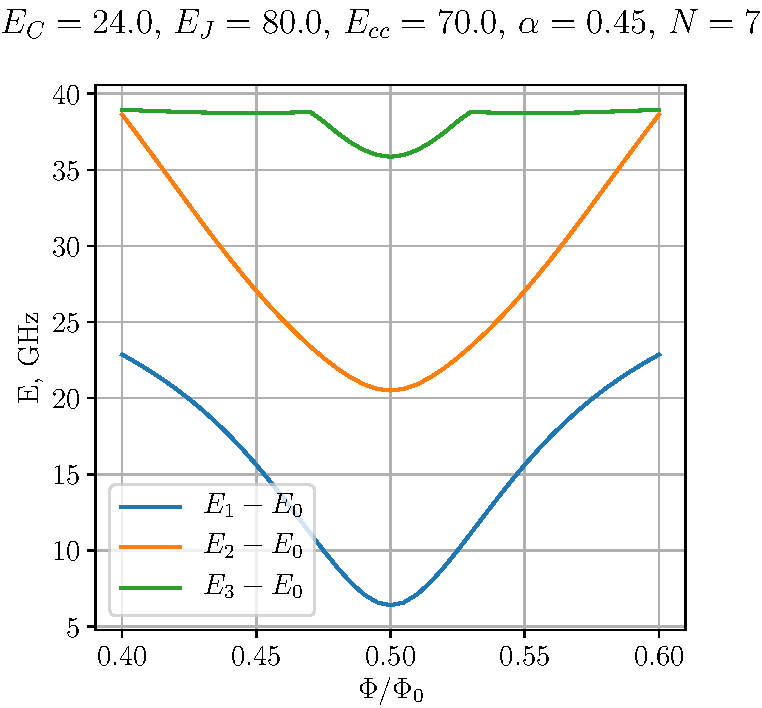
\includegraphics[width=0.55\textwidth]{images/4jj_qubit_spectra_side_coupled}}
		
		\hfill
	}
	\caption[Схема потокового кубита с четырьмя джозефсоновскими переходами и его спектр]{Потоковый кубит с 4 переходами: a) Эквивалентная схема кубита, связанного с волноводом.  б) Спектр кубита: энергии переходов из основного состояния в зависимости от внешнего потока через петлю для некоторых типичных значений параметров. Значения $E_C, E_J, E_{cc}$~приведены в ГГц. }
	\label{img: 4jj_flux_q}
\end{figure}

\begin{figure}[h]
	\centering
	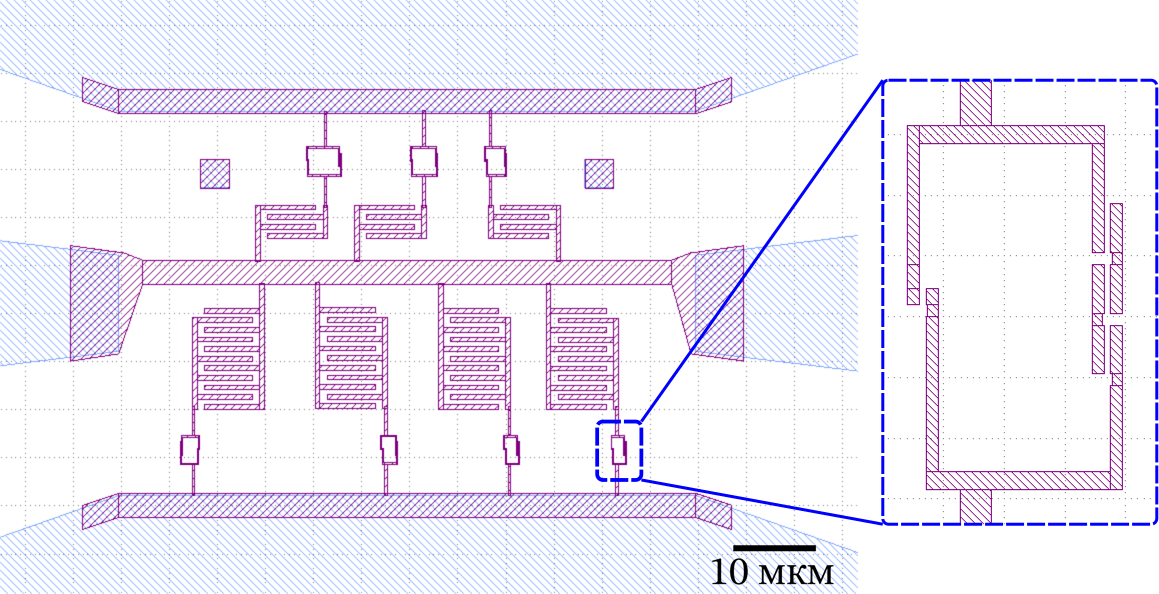
\includegraphics[width=1\textwidth]{images/fig_qubits_design.png}
	\caption{Дизайн потоковых кубитов, параллельно связанных с копланарной линией при помощи емкостей. Параметр $\alpha=0.36,0.45$, площади петель от 5 до 40 мкм$^2$, связывающие емкости $C_c=2.2,6.4$~фФ }
	\label{img: 4jj_side}
\end{figure} 
\begin{figure}[h]
	\centering
	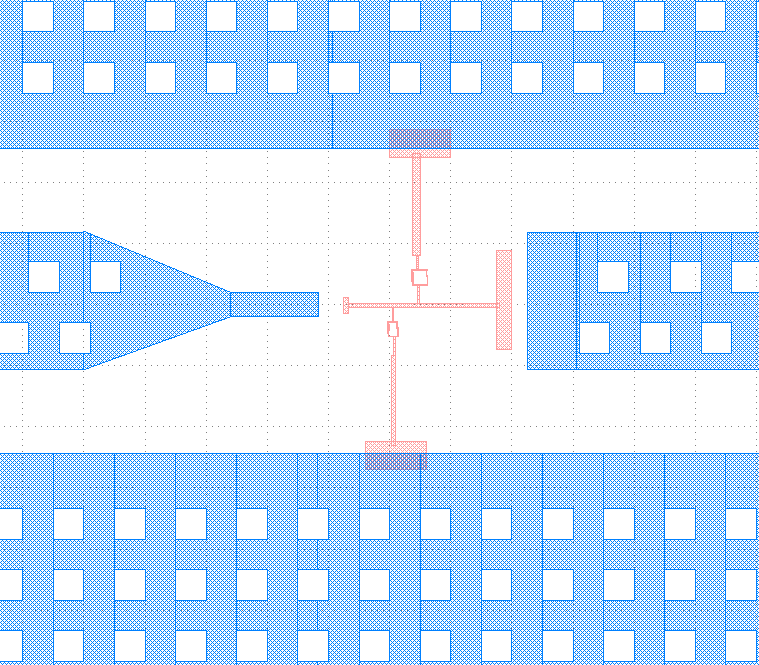
\includegraphics[width=0.6\textwidth]{images/SPS_design2.png}
	\caption{Дизайн 4-переходных потоковых кубитов, связанных с двумя полубесконечными копланарными линиями. Параметр $\alpha=0.4$, площади петель 14.2 и 21.2 мкм$^2$, связывающие емкости $C_{in}=0.24, C_{out} = 2.2 $~фФ }
	\label{fig: qubits_sps}
\end{figure} 
Для последующей фабрикации были рассчитаны и отрисованы дизайны экспериментальные образцов: дизайн на рис. \ref{fig: qubits_sps} реализует режим прямой связи (англ. \textit{direct coupling}), а дизайн образца на рис.
\ref{img: 4jj_side} --- режим параллельной связи (англ. \textit{side coupling}) кубита к излучению. Выбор схем не оказывает прямого влияния на процесс фабрикации кубитов. Остановимся на дизайне с параллельной связью. Спроектированный дизайн содержат кубиты с 4-мя джозефсоновскими переходами, три из которых имеют одинаковую площадь $200\times800$~нм, а еще один переход в $\alpha\approx0.4$ раз меньше остальных. Переходы будут формироваться при напылении через маску, повторяющую дизайн, под различными углами, примерно $\pm11^\circ$ Кубит связывается с электромагнитным полем, распространяющемся в копланарном волноводе, посредством связывающей емкости $C_c=2.2$ или $6.4$~фФ. Эта емкость фактически оказывается подключенной к земле через небольшое активное сопротивление $Z_0$ и поэтому оказывает шунтирующий эффект на $\alpha$-переход, необходимый для уменьшения чувствительности потокового кубита как к потоковым, так и зарядовым шумам. Более подробно, шунтирование~$\alpha$-перехода, добавляясь к внутренней емкости перехода $C_j=2$-$3$~фФ, уменьшает зарядовую энергию. Это приводит к тому, чтоб есть возможность уменьшить джозефсоновские энергии переходов, сохраняя при этом частоты кубитов. Это понижает чувствительность кубита к магнитному полю и, соответственнно, к шуму магнитного потока, что при прочих равных условиях может увеличить время когерентности. Влияние шунтирующей емкости на спектры 3-переходного потокового кубита отражено на Рис. \ref{fig: 3jj_spectra}. Также влияние емкостного шунта на потоковые кубиты детально исследовано в работе \cite{yan2016flux}, как теоретически, так и экспериментально. При существенно б$\acute{\text{о}}$льших значениях шунтирующей емкости порядка $50$ фФ кубит, фактически, становится слабо ангармоничным осциллятором с небольшими следами <<двухъямности>>, ангармонизм падает значительно ниже 1 ГГц. Это перспективно для достижения больших времен когерентности, но нежелательно для выполнения поставленных в диссертации задач. Для иллюстрации изложенных закономерностей, на рис. \ref{img: 4jj_flux_q}\subcaptionref*{img: 4jj_fluxQ_spectrum} приведены типичные зависимости энергии уровней от внешнего магнитного поля (спектры) кубитов для реалистичного набора параметров, полученные при помощи численной диагонализации полного гамильтониана в зарядовом базисе. В рабочем режиме частота кубита $\omega_0=E_e-E_g/\hbar$ должна находиться в пределах 2-10 ГГц, что обусловлено частотными диапазонами криогенных усилителей и изоляторов (подробнее об этом ниже).

Магнитное поле через кубиты обычно подается при помощи сверхпроводящего соленоида, который намотан на держатель и будет показан ниже. Однако, такой способ не может обеспечить индивидуальную перестройку частоты отдельных кубитов. Поэтому в ряде случаев полезно иметь возможность менять поток через потоковый кубит (или через СКВИД кубита-трансмона) при помощи дополнительной потоковой линии на чипе. Потоковая линия представляет собой копланарный волновод, который закорочен на землю вблизи той петли, поток в которой необходимо менять. Ток, текущий в потоковой линии, создает локальное магнитное поле, которое используется для перестройки магнитного потока. 

\begin{figure}[htb]\center
	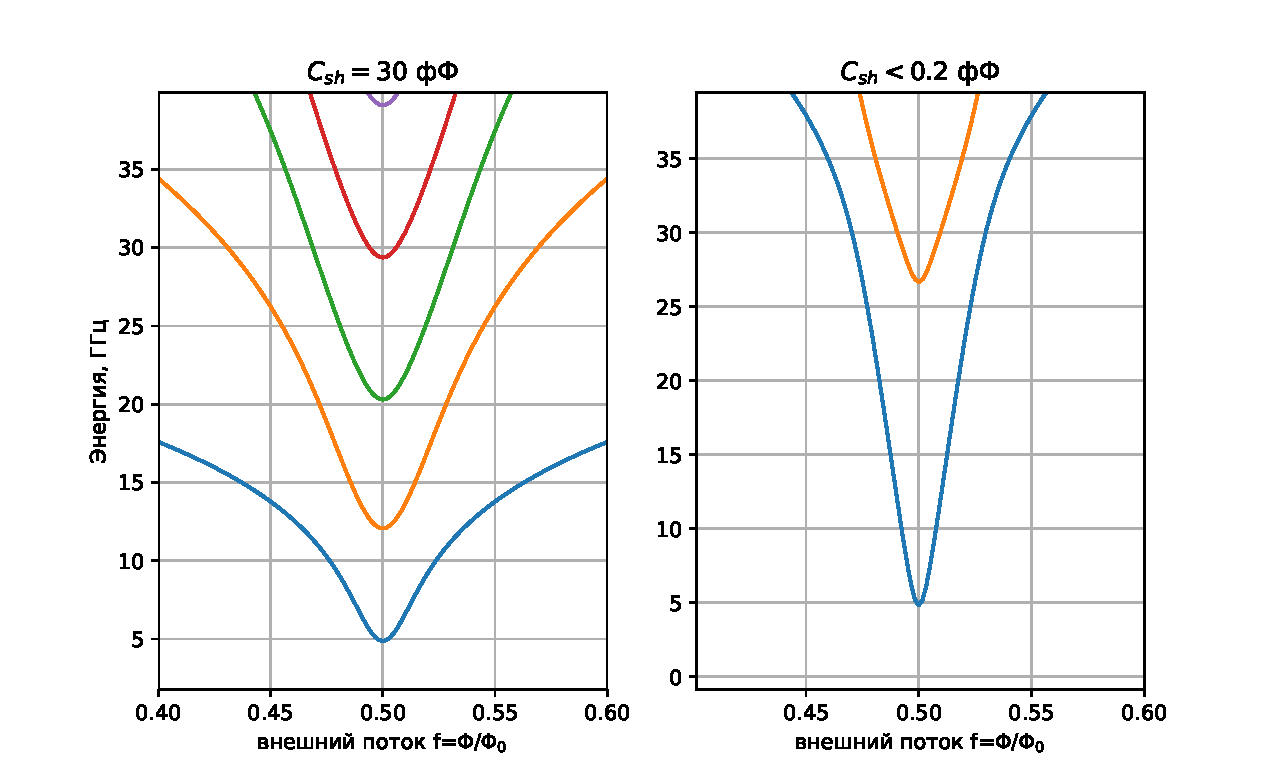
\includegraphics[width=1\textwidth]{images/3jj_spectra.pdf} \hfill
	\caption[Влияение шунтирующей емкости на спектры потоковых кубитов]{Рассчитанные спектры $E_n-E_0$ потоковых кубитов с тремя джозефсоновскими переходами с учетом влияния шунтирующей емкости $C_{sh}$ на $\alpha$-переходе. В обоих случаях $E_c = 25$~ГГц, $E_j=170$~ГГц. Левая панель: спектр для параметров $C_{sh} = 30$~фФ, $\alpha=0.5$. Правая панель: спектр для параметров $C_{sh} \approx 0.1$~фФ, $\alpha=0.69$. Как можно заметить, при равных параметрах переходов (что соответствует одинаковому процессу окисления) большая шунтирующая емкость сглаживает спектр и делает кубит не столь чувствительным к дефазировке по потоку, при этом ангармонизм еще достаточно велик (1-2 ГГц). В случае отсутствия шунта, приходится понижать частоту перехода 0-1 при помощи увеличения $\alpha$, однако, при смещении от оптимальной точки $f=0.5$ производная энергии по потоку значительно увеличивается, и такой кубит гораздо сильнее подвержен дефазировке. Кроме того, при отсутствии шунта верхние уровни имеют слишком высокую частоту и недоступны для использования.}
	\label{fig: 3jj_spectra}
\end{figure}
\subsection{Маршрутная карта для изготовления образцов}

Образцы кубитов изготавливались в условиях чистой комнаты класса ISO-5 (не более 1000 пылинок размером более 1 мкм в 1 м$^3$ воздуха). Маршрутная карта включает следующие процедуры:
\begin{enumerate}
	\item Отмывка подложки из высокоомного недопированного кремния 
	\begin{itemize}
	  \item дистилированная вода+ультразвук, 2 мин
	  \item IPA, 10 сек
	  \item NMP, 150 $^\circ$C, 5 мин
	  \item RCA-1+ультразвук, 80 $^\circ$C, 2 мин 
	\end{itemize}
	\item Нанесение копланарной линии
	\begin{itemize}
		\item нанесение резиста LOR-5B 3000 об/мин, 180$^\circ$C, 7 мин;
		\item нанесение резиста S1813 4000 об/мин, 115$^\circ$C 7 мин;
		\item фотолитография на литографе Heidelberg 8 мВ, 80%;
		\item проявка KOH 45 сек;
		\item напыление 100 нм пленки Al (Plassys), 0.2 нм/c; 
		\item лифт-офф NMP+ультразвук 100$^\circ$C, 5 мин;
	\end{itemize}
	\item Нанесение туннельных контактов
		\begin{itemize}
			\item нанесение резиста Copolymer/MMA 9\% 3000 об/мин, 150$^\circ$C, 5 мин;
			\item нанесение резиста ARP 6200.04 4500 об/мин, 150 $^\circ$C 5 мин;
			\item электронная литография на литографе Crestec CABL 9000 160 pA, 1 мкс/точка;
			\item проявка AR 600-546 1 мин, IPA 30 с, дистилированная вода 30 сек;
			\item напыление нижней пленки Al толщиной 25 нм под углом $+11^\circ$ (в установке Plassys), скорость напыления 0.2 нм/c.
			\item Промежуточное окисление при давлении 2 мБар в течение 5 мин; 
			\item напыление верхней пленки Al толщиной 45 нм под углом $-11^\circ$, 0.2 нм/c.
			\item лифт-офф NMP+ультразвук 100$^\circ$C, 5 мин;
		\end{itemize}
\end{enumerate}

Представленный процесс может быть изменен или дополнен. В ряде случаев перед напылением джозефсоновских контактов требуется удалить естественный слой оксида с алюминиевой пленки, для этого используется травление ионами Ar при помощи пушки. Типичные параметры: ускоряющее напряжение 80В, ток эмиссии 20 мА, время 2 минуты.

Согласно даннной маршрутной карте были изготовлены образцы. При рассмотрении в оптическом микроскопе была проведена инспекция микронных структур на соответствие размерам, задаваемым в дизайне, см.~Рис. \ref{img: line_opt_control}.  При помощи СЭМ сделаны изображения изготовленных кубитов, см.~Рис. \ref{img: qubits_sem}. Можно наблюдать сформированные переходы, размеры которых близки к заложенным в дизайн значениям. Последний шаг проверки вновь сделанных образцов --- измерение нормального сопротиления тестового перехода или СКВИДа при помощи зондовой станции. Для переходов 200x800 получены значения в диапазоне $R_n=2.1-2.4$~кОм. Если предположить, что при падении температуры от комнатной до $T_c$ сопротивление уменьшается в 3 раза, то для джозефсоновской энергии имеем $E_J/h \approx 160$~ГГц. Однако, эта оценка является весьма неточной, поскольку точное значение нормального сопротивления джозефсоновского контакта вблизи сверхпроводящего перехода неизвестно, хотя в принципе может быть оценено из ВАХ отдельных переходов. 
\begin{figure}[htb]\center
	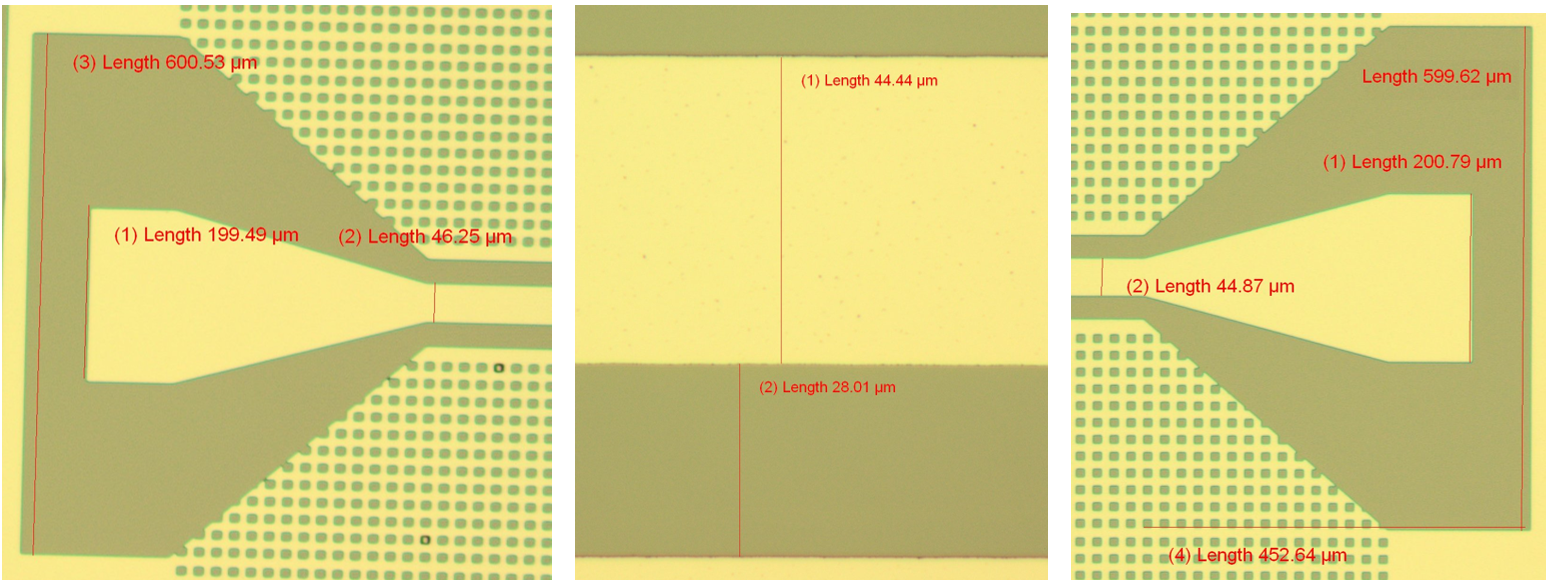
\includegraphics[width=1\textwidth]{line_opt_control.png} \hfill
	\caption[Контроль размеров микронных структур в оптическом микроскопе]{Контроль поперечных размеров копланарной линии  и контактных площадок при помощи оптического микроскопа. Размеры отклоняются от заложенных в дизайн значений не более чем на 1 мкм.}
	\label{img: line_opt_control}
\end{figure}

\begin{figure}[htb]\center
	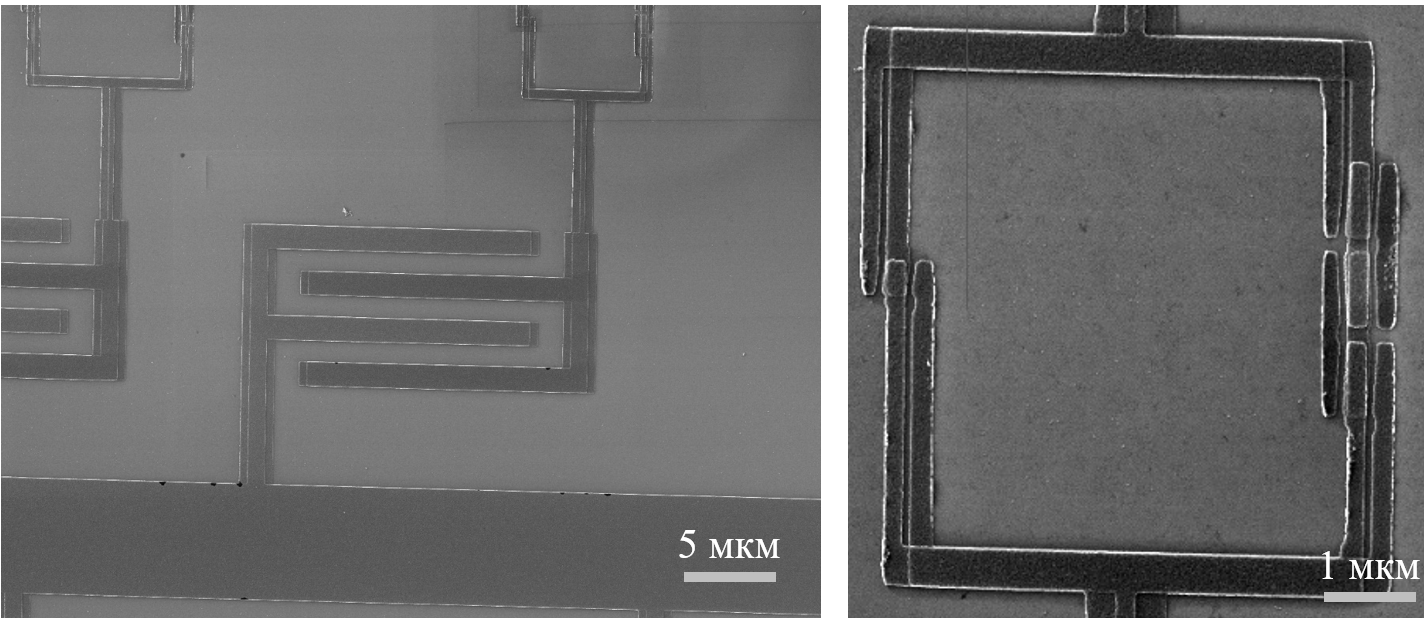
\includegraphics[width=1\textwidth]{qubits.png} \hfill
	\caption{Изображение связывающей емкости и кубита в сканирующем электронном микроскопе (СЭМ)}  
	\label{img: qubits_sem}
\end{figure}
Следующий шаг --- сборка измерительной схемы внутри криостата растворения и помещение в неё образца с кубитами для последующих измерений. 
\section{Схема подключения кубитов в линии}
После того, как чип с волноводом и кубитами изготовлен, необходимо  собрать измерительную схему, которая позволит осуществить экспериент по измерению нелинейного рассеяния на кубите. Для размещения чипов внутри криостата необходимо:
\begin{itemize}
	\item{разместить чип с кубитом внутри печатной платы, закрепленной на внутренней части высокочастотного низкотемпературного держателя;}
	\item{приклеить чип и осуществить ультразвуковую разварку контактных площадок высокочастотных линий на чипе к отрезкам копланарных линий печатной платы;}
	\item{собрать высоко- и низкочастотные входные и высокочастотные выходные линии по всей длине криостата, начиная от фланца с температурой 50 К и заканчивая ответной частью держателя на фланце с базовой температурой;}
	\item{вставить держатель с платой в его ответную часть, закрепляемую на нижней ступени рефрижератора;}
	\item{при помощи тестера определить сопротивления между центральными жилами сигнальных проводов и землей и между входной и выходной линиями держателя, подходящими к волноводу на чипе;}
	\item{соединить разьемы линий с разьемами держателя соотвественно;}
	\item{протестировать высокочастотное пропускание волновода, подключив входную и выходную линии к ВАЦ;}
	\item{в случае хорошего прохождения сигнала, загрузка считается успешной и можно приступить к охлаждению криостата.}
\end{itemize} 
Рассмотрим некоторые из этих манипуляций более подробно и опишем те свойства, которыми должна обладать измерительная схема для правильного функционирования образца. 
\subsection{Устройство держателя}

Первое и самое очевидное условие работы кубитов --- возможность охлаждения чипа до базовой температуры рефрижератора, которая равна 15-20 мК. Такую же температуру должна иметь и печатная плата, на которой размещается чип, и та часть держателя (бобышка), которая контактирует с печатной платой и кубитным чипом. Это налагает очевидные ограничения на те материалы, из которых может состоять держатель. Стальные сплавы имеют крайне низкую теплопроводность при температурах менее 1 К. Аналогичное можно сказать о любом сверхпроводнике, охлажденном ниже $T_c$ --- отсутствие свободных носителей тока ухудшает возможность переносить тепло. Поэтому все компоненты держателя должны быть изготовлены из меди (в крайнем случае из латуни). Наилучшую теплопроводность при температурах ниже 100 мК обеспечивает бескислородна медь, но использование обычной чистой меди (марка М1) практически не влияет на скорость охлаждения. 

Держатель состоит из нескольких обязательных частей --- печатная плата, бобышка, ответная часть, крепление к фланцу, магнитный и сверхпроводящий экраны и различные вспомогательные элементы. 

Печатная плата изготавливается из высокочастотного стека. Стек состоит из двух медных слоев толщиной порядка 100 мкм, разделенных диэлектриком с малыми потерями, например, Arlon AD-1000. Плата имеет сквозное отверстие для размещения чипа. К краям отверстия подходят копланарные линии, которые расходятся в радиальных направлениях и заканчиваются возле краев платы специальными расширениями, на которые впоследствии запаиваются высокочастотные разъемы. Плата предусматривает размещение от 4 до 12 SMP-разьемов типа <<папа>>, центральная жила которых запаивается на центральную дорожку копланарных высокочастотных линий. В эти разъемы затем вставляются коаксиальные провода с ответными SMP-разъемами, которые будут крепиться на ответной части держателя. 

Печатая плата плотно прикручивается к бобышке для обеспечения хорошего высокочастотного электрического контакта между нижней металлизацией печатной платы и объемом бобышки. Важный атрибут бобышки --- наличие прямоугольной полости в месте крепления чипа. Полость повторяет форму чипа и имеет глубину 5-7 мм. Она нужна для смещения резонансных объемных мод кремниевого чипа в область высоких частот, что особенно актуально для чипов больших размеров. Поскольку диэлектрическая проницаемость кремния достаточно велика: $\varepsilon=11.7$, то для чипа с продольным размером $a=10$ мм первая объемная мода имеет частоту $f_1 = c/2a\sqrt{\varepsilon}=4.33$~ГГц. Эта частота находится точно в середине рабочей области и потому может легко возбуждаться, если попадает в резонанс с сигналом в копланарной линии на поверхности чипа. Однако, если добавить полость под чипом и рассмотреть вновь получившийся объемный резонатор, то эффективная $\varepsilon$ упадет в несколько раз, и объемные моды перестанут оказывать прямое влияние на распространение сигнала по копланарным линиям на чипе. 

Бобышка с печатной платой вставляется в ответную часть держателя. Ответная часть представляет из себя цилиндрическую полость без дна (дном служит бобышка). В верхнем торце ответной части располагаются отверстия, которые располагаются точно над SMP-разъемами печатной платы. Через эти отверстия проходят провода, подключающиеся к SMP-разъемам. В середине ответной части имеется ушко, за которое она подвешивается к штанге длиной около 30 см. Штанга, в свою очередь, прикрепляется к крепежному фланцу. Крепежный фланец имеет сквозные отверстия для SMA-переходников и крепления для магнитного и сверхпроводящего экранов. SMA-переходники накручиваются на сквозные отверстия. На внутренние разъемы переходников накручиваются провода, идущие к печатной плате, а на внешние разъемы переходников приходят (с внешних разъемов уходят) входные (выходные) коаксиальные линии. Также в фланце имеется отверстие для пары проводов, запитывающих сверхпроводящий соленоид. Соленоид наматывается на боковую поверхность ответной части держателя, а контакты выводятся через отверстие и подключаются к линиям постоянного тока, выходящим на фланец с базовой температурой.

Поскольку кубиты чувствительны к внешнему магнитному полю, чипы необходимо экранировать от магнитного поля Земли и от другого паразитного магнитного поля шума, которое создают электрические приборы. Для этого на фланец надевается цилиндрический сверхпроводящий экран. Этот экран будет захватывать магнитное поле благодаря эффекту Мейснера. Имеется возможность дополнительно уменьшить поле, которое будет вытесняться сверхпроводящим экраном. Для этого поверх сверхпроводящего экрана надевается еще один экран из криогенного пермаллоя (Cryoperm) - мягкого магнитного металла с очень большим значением магнитной восприимчивости $\mu \approx 10^5$. Силовые линии магнитного поля концентрируются внутри криоперма, а магнитное поле внутри экрана будет ослаблено (в идеале в $\mu$ раз, на практике далеко не так эффективно из-за того, что экран не имеет крышки.). Описанное решение является относительно стандартным и с теми или иными модификациями (например, использование второго криопермового экрана вместо сверхпроводящего) используется во многих исследовательских группах, работающих со сверхпроводящими кубитами. Непосредственная проверка эффективности ослабления внешнего магнитного поля не проводилась, но в ходе экспериментов, описываемых в данной работе, не возникало явных указаний на критически значимые магнитные шумы. 

Мы завершили общее описание держателя. Теперь необходимо изложить требования, которые предъявлются к схеме измерения кубитов.

\subsection{Требования к измерительной схеме}
Схема измерения кубитов в линии включает в себя низкотемпературную часть внутри криостата растворения и управляющую электронику при комнатной температуре, которая подключается к криостату и управляется при помощи компьютера. Низкотемпературная часть схемы изображена на Рис. \ref{fig: schemes} для случая параллельной связи (неразрывная линия с кубитом) и для случая прямой связи (кубит связан с двумя полубесконечными линиями). 
\begin{figure}[htb]\centering
	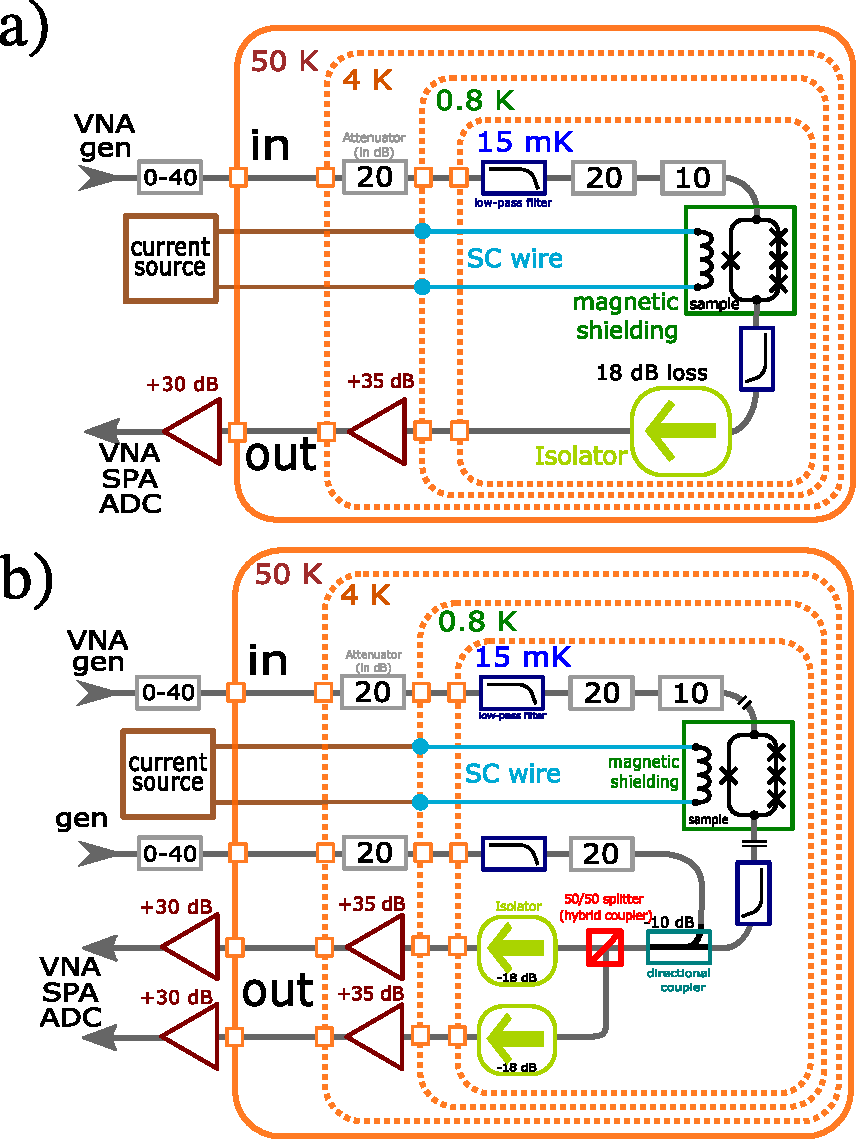
\includegraphics[width=0.8\textwidth]{images/meas_schemes_2.pdf} \hfill
	\caption{Низкотемпературная часть измерительных схем. а) --- схема для кубита в линии (параллельная связь), б) --- схема для кубита, связанного с двумя полупространствами (прямая связь) }
	\label{fig: schemes}
\end{figure}

Сначала обсудим общие свойства изображенных схем. На Рис. \ref{fig: schemes} оранжевыми пунктирными линиями выделены различные ступени криостата растворения. Держатель с чипом располагается внутри магнитного экрана при базовой температуре (примерно 15 мК). К нему подходят входные высокочастотные коаксиальные линии внутри криостата (на Рис. \ref{fig: schemes} обозначены серым цветом). На каждой ступени в линии включаются аттенюаторы с различным номиналом (от 0 до 20 дБ ослабления) для термализации теплового шума, который распространяется далее по линии. Выходной сигнал, как правило, имеет очень малую мощность, и необходимо обеспечить минимальные потери до первого усиления. По этой причине выходные коаксиальные линии  делаются сверпроводящими от чипа до низкотемпературных усилителей (коричневые треугольники), располагающихся на 4К-фланце (фланце с температурой около 4 кельвин). На эти линии нельзя поставить аттенюаторы для ослабления теплового шума. Поэтому защитить чип от тепловой радиации можно лишь при помощи магнитных изоляторов (изображены на схемах зелеными стрелками) --- диодов для высокочастотного сигнала, которые почти не ослабляют СВЧ-сигнал в прямом направлении, но дают примерно 18-20 дБ в обратном направлении.  Низкочастотные линии (на Рис. \ref{fig: schemes} коричневые/голубые) представляют из себя витые пары, которые подключаются к соленоиду, а также подводят питание для радиочастотных переключателей, которые располагаются на базовой ступени криостата и дают возможность подключать к одной выходной линии несколько входных (на схемах переключатели не показаны, поскольку в описываемых далее экспериментах они не использовались).

Как уже упоминалось ранее, кубит должен находиться в тепловом равновесии при базовой температуре криостата 15 мК. Ранее мы пояснили, что хороший тепловой контакт чипа с держателем является одним из условий, способствущих хорошему охлаждению кубита. Однако влияние на состяоние кубита имеет не столько фононная температура чипа (которая действительно близка к базовой), сколько температура электронной подсистемы. Условие эффективной термализации электронной системы сверхпроводящей цепи на чипе --- эффективное ослабление теплового шума, который испускают электронные приборы на комнатной температуре. Правильная расстановка аттенюаторов без каких-либо дополнительных действий снижает электронную температуру до 50 мК, что можно подтвердить из независимого определения температуры при помощи, например, термометра на основе эффекта кулоновской блокады \cite{Meschke2004}. Для дальнейшего понижения температуры требуется установка ИК-фильтров \cite{Longobardi2013}, предотвращающих распространение фотонов частотами от 20 до нескольких сотен ГГц в коаксиальных линиях. Для описанных в работе измерений ИК-фильтры не применялись. Рассмотрим более подробно, как аттенюаторы ослабляют тепловой шум, проникающий в криостат растворения.

\subsection{Ослабление теплового шума}
Любой активный электронный прибор (например, СВЧ-генератор), располагающийся на комнатной температуре и имеющий выходное сопротивление $Z_0$, будет выдавать на выход некоторый шум. В целом, электронный шум включает в себя дробовой шум, который зависит от протекающего тока, низкочастотный шум $1/f$, характерный для всех типов полупроводниковых электронных приборов, а также тепловой шум. Спектральные плотности дробового шума и фликер-шума $1/f$ при комнатной температуре пренебрежимы по сравнению со спектральной плотностью теплового шума Джонсона-Найквиста, которую можно записать как:
\begin{equation}
S_V(T, \omega) =\frac{2\hbar \omega Z_0}{1-\exp\left(-\hbar\omega/k_bT\right)}
\label{eq: J-N}
\end{equation}

При высоких температурах $\hbar \omega \ll k_b T $. Тогда из \eqref{eq: J-N} получаем классическое выражение $S_V(\omega) = 2k_bTZ_0$, а значит, на начальных стадиях при $T \gg $ 1~К тепловой шум нужно ослаблять пропорционально температуре ступени. Однако, при более низких температурах это простое правило уже не работает, и ослаблять тепловой шум нужно значительно сильнее. Чтоб пояснить это, отметим, что спектральная плотность шума напряжения \eqref{eq: J-N} может быть рассчитана как для положительных, так и для отрицательных частот. Разница особенно заметна при нулевой температуре: $S_V(0,\ {\omega\! <\! 0})=0$, тогда как $S_V(0,\ {\omega\! >\! 0})=2Z_0 \hbar\omega$. Физический смысл этого различия можно пояснить, вычислив скорости возбуждения и релаксации двухуровневой квантовой системы под действием шума \cite{schoelkopf2003qubits}. Если кубит взаимодействует с внешним напряжением в дипольном приближении $H_{int} = A V(t) \sigma_x$, то из теории возмущений можно получить:
\begin{equation}
\Gamma_\downarrow = \frac{A^2}{\hbar^2}S_V(+\omega_q), \quad \Gamma_\uparrow = \frac{A^2}{\hbar^2}S_V(-\omega_q).
\end{equation}
\begin{figure}[h]\centering
	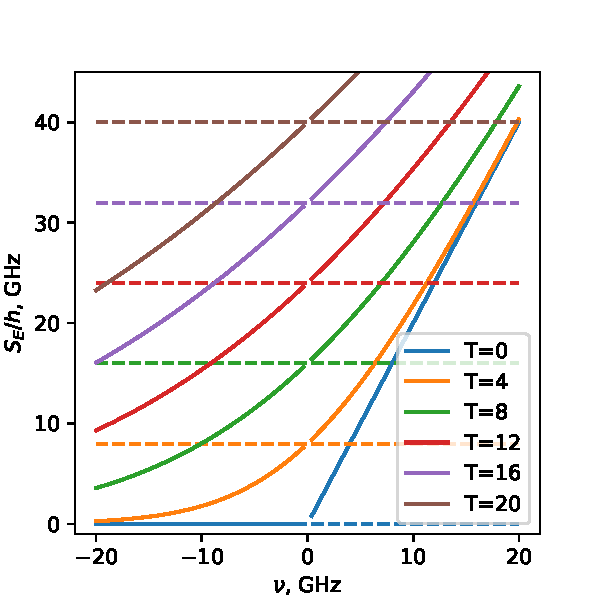
\includegraphics[width=0.7\textwidth]{QN_spectrum.pdf} \hfill
	\caption[Спектральная плотность флуктуаций напряжения]{Спектральная плотность флуктуаций напряжения в зависимости от нормированной температуры $T/k_b h$ и частоты $\nu=\omega/2\pi$ (в ГГц) согласно выражению \eqref{eq: J-N}. Пунктирная линия отмечает классическое выражение для спектральной плотности $S_V = 2 k_b T$. }
	\label{img: S_V}
\end{figure}
Таким образом, шум на отрицательных частотах может поглощаться и вызывать возбуждение системы. Наоборот, спонтанную релаксацию возбужденного кубита (или резонатора в квантовом режиме) вызывает шум на положительных частотах. Поэтому для эффективной термализации кубита частотой $\omega_q$, расположенного при базовой температуре $T_b$ нужно ослабить шум верхних ступеней до уровня $S_V(T_b, -\omega_q)$. 

Точный расчет остаточного числа фотонов, достигающего базового фланца при различных номинальных значениях аттенюаторов, показывает \cite{krinner2019engineering}, что наиболее оптимальная конфигурация с точки зрения ослабления остаточного шума предусматривает расположение по 20 дБ ослабления на 4К-ступени, на промежуточном фланце температурой около 100 мК между фланцем Still температурой 0.8 К и базовым фланцем температурой 10-15 мК), и на базовом фланце --- всего 60 дБ ослабления. Однако, чтоб иметь возможность сильно увеличивать амплитуду драйва, в экспериментах использовалось 40-50 дБ ослабления за счет уменьшения номинала аттенюатора на ступени с температурой 100 мК до 10 дБ, либо полного его снятия.

\subsection{Усиление рассеянного сигнала}
\label{sec: amplif}
Как выяснено в предыдущем подразделе, после прохождения входной линии тепловой шум  ослабляется для предотвращения нежелательной зачеселенности кубита. Аналогичным образом ослабляется и управляющий кубитом когерентный сигнал. Как ясно из представленных в разделе \ref{sec: microwave qo} расчетов, характер действия поля на кубит, и соотвественно, характер рассеяния когерентного сигнала определяются амплитудой Раби $\Omega$ и отстройкой от кубита $\delta\omega$. На выходе из волновода к исходному сигналу добавляется рассеянное на кубите поле, определяемое выражением \eqref{eq: sc_field}. Эквивалентную мощность этого сигнала можно оценить как:
\begin{equation}
P_{sc} = \frac{|V_{sc}|^2}{2Z_0} \approx \frac{(\hbar \Gamma_1/2e)^2}{2Z_0} \approx -155 \text{ дБм}.
\label{eq: P_sc}
\end{equation}
Оценка сделана в приближении $\mu\!\approx\!2e$ и для $\Gamma_1\!=\!2\text{ МГц.}$. Отсюда можно сделать два вывода. Во-первых, перед измерением столь малый сигнал необходимо значительно усилить, поскольку типичные ВАЦ и СА могут обнаруживать сигналы мощностью около -100 дБм. Во-вторых, очевидно, что необходимо использовать малошумящие низкотемпературные усилители, поскольку эквивалентная температура, соотвествующая мощности \eqref{eq: P_sc} в полосе $\Gamma_1$, примерно равна:
\begin{equation}
T_{eq} = \frac{P_{sc}}{4k_b\Gamma_1} = 2.8 \text{ мК}. 
\end{equation}
В экспериментальной установке в качестве первого каскада усиления используются доступные в коммерческих целях усилители фирмы Low Noise Factory с эквивалентной шумовой температурой 2-4 К, так что даже в случае их использования отношение <<сигнал-шум>> по порядку величины не превышает 1/100. Эти усилители располагаются на ступени с температурой 4 К. Дальнейшее усиление осуществляется при помощи комнатных высокочастотных усилителей Mini Circuits ZVA-183+ или их аналогов. Общее усиление составляет примерно 80-100 дБ при использовании узкополосных приборов (например, при измерении стационарного поля) и 120-140 дБ при использовании высокочастотных ЦАП. Это вызвано тем, что битность высокочастотных ЦАП ограничена, и для качественной оцифровки требуется сигнал более высокой амплитуды.

\section{Спектроскопия кубитов}
\label{sec: spectr}

Как выяснено в разделе \ref{subsec: flux_q}, частота потокового кубита перестраивается магнитным потоком, пронизывающим контур кубита. Трансмон со СКВИДом вместо джозефсоновского перехода также перестраивается магнитным полем. По этой причине первичным измерением потокового (как и практически любого другого) кубита в волноводе является однотоновая спектроскопия. Входная и выходная линия подключаются к ВАЦ, после чего измеряется коэффициент пропускания $S_{21}$ в зависимости от тока в катушке или в потоковой линии. Это позволяет найти частоту кубита при различных потоках, в частности, найти оптимальные по потоку точки, если это необходимо для дальнейших измерений. 

На Рис.~\ref{img: circlefit} изображена частотная характеристика кубита в линии при базовой температуре, полученная при помощи ВАЦ в режиме $\Omega \ll \Gamma_1$. В случае очень слабой накачки поведение кубита в линии ничем не отличается от резонатора, включенного параллельно линии по схеме типа <<notch-порт>>. Детальная модель частотной характеристики для таких резонаторов была построена в работах \cite{gao2008physics,Khalil}. В рамках этой модели показано, что пропускание через такой резонатор представляет собой ассимметричный лоренцевский пик, описываемый выражением:
\begin{equation}
S_{21}^\text{notch}(f) = \underbrace{\vphantom{\frac{Q_l e^{i\phi}}{1+2iQ_l\left(f/f_r -1  \right)}}  a e^{i\alpha} e^{-2\pi i f \tau}}_{\text{окружение}} \underbrace{\left[ 1 - \frac{\left(Q_l/ |Q_c|\right) ~ e^{i\phi}}{1+2iQ_l\left(f/f_r -1  \right)}  \right]}_{\text{идеальный резонатор}}\,.
\label{eq:S21model}
\end{equation}
Опишем некоторые свойства модели:
\begin{itemize}
	\item {модель учитывает частотно-зависимый набег фазы $-2\pi i f \tau$, который возникает из-за задержки распространения сигнала через тракт $\tau$;} 
	\item {связь к линии характеризуется при помощи добротности связи $Q_c$ (комплексная величина);}
	\item {модель учитывает дополнительный фазовый сдвиг $i\phi$ комплексного сигнала, соотвествующего пику резонатора на частоте резонанса $f_r$. Этот сдвиг возникает из-за индуктивного импеданса бондирующих проводов, а также из-за несогласований на переходниках по ходу коаксиальных линий;}
    \item {внутренние потери в резонаторе описываются внутренней добротностью $Q_i$, которая может быть выражена через полную (нагруженную) добротность резонатора в линии $Q_l$:
    	\begin{equation}
    	Q_i^{-1} = Q_l^{-1} - \text{Re}\left\{ Q_c^{-1} \right\}.
    	\end{equation}}
\end{itemize}
\begin{figure}[h]\centering
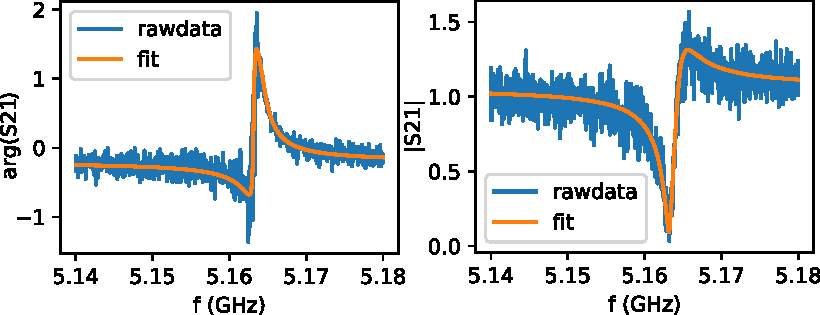
\includegraphics[width=1\textwidth]{qubit_circlefi_2_edit.pdf} \hfill
\caption[Пропускание волновода с кубитом]{Частотная характеристика коэффициента прохождения $S_{21}(f)$ высокочастотного маломощного сигнала через волновод с кубитом. Измеренный сигнал нормирован на фоновое пропускание, измеренное при большой мощности, либо же при значительной отстройке кубита. Данные подогнаны при помощи модели резонатора в линии (см. основной текст), параметры фита отображены в Табл.~\ref{Tab1}.}
\label{img: circlefit}
\end{figure} 
\begin{table} [htbp]
	\centering
	\changecaptionwidth\captionwidth{15cm}
	\caption{Параметры модели пропускания резонатора}\label{Tab1}%
	\begin{tabular}{| p{2.2cm} | p{3cm} | p{3cm}l |}
		\hline
		\hline
		Параметр   & \centering Значение & \centering Ошибка & \\
		\hline
		$Q_i$ &\centering  20275  &\centering 2225 & \\
		$Q_c$ &\centering  2448  &\centering  49 &\\
		$f_r$, Гц &\centering  5.164$\cdot10^9$  &\centering 4.43$\cdot10^4$ &\\
		$\phi$, рад &\centering  -0.681  &\centering  0.025 & \\
		\hline
		\hline
	\end{tabular}
\end{table}
Измеренный коэффициент $S_{21}$ был подогнан при помощи репозитория \verb|circlefit|, разработанного в \cite{Probst_circlefit}. Результаты измерения пропускания кубита с наложенной линией подгонки изображены на Рис. \ref{img: circlefit}. Можно заметить, что модель хорошо описывает экспериментальные данные. Результат подгонки дает значения $ Q_i, Q_c, f_r \text{ (для кубита уместнее обозначение }f_q)$ и других параметров, которые приведены в Табл.~\ref{Tab1}.

Добротность связи кубита с линией можно связать со скоростью излучательной релаксации:  $\Gamma^r_1/2\pi= f_q/Q_c = 2.1$~МГц на основе данных из Табл.~\ref{Tab1}. Внутренняя добротность можно списать на всевозможные причины, по которым когерентный сигнал не достигает ВАЦ после рассеяния на кубите. Это безызлучательная релаксация, в которую можно включить потери в кубите и релаксацию в какие-либо паразитные моды, а также чистая дефазировка: $\left(\Gamma_1^{nr} + 2\Gamma_\varphi \right)\!/2\pi = f_q/Q_i = 255\text{ кГц}$, опять же на основе Табл.~\ref{Tab1}.

Однотоновая спектроскопия представляет собой измерение, при котором линия пропускания кубита, показанная на Рис.~\ref{img: circlefit}, измеряется при различных значениях магнитного потока в катушке или в токовой линии, при этом частоа кубита перестраивается. В результате получаются спектры потоковых 
кубитов, пример которых приведен на Рис.~\ref{img: singletone}. 

\begin{figure}[h]\centering
	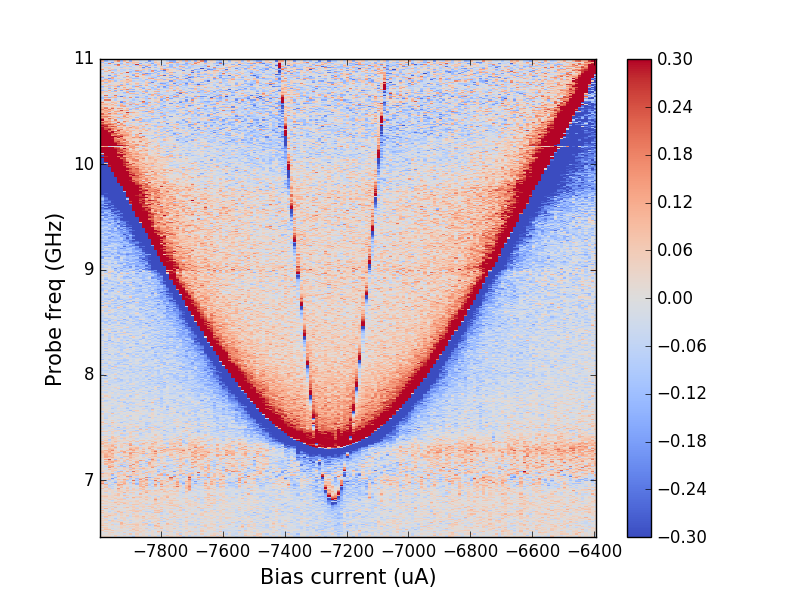
\includegraphics[width=0.9\textwidth]{FluxQ_spectra4_both.png} \hfill
	\caption[Измеренные спектры потоковых кубитов]{Однотоновая спектроскопия потоковых кубитов: $\arg\left(S_{21}(f) \right)$ в зависимости от тока через катушку держателя. Можно различить спектры двух кубитов с различным значением $\Gamma_1$, соотвествующие различным связывающим емкостям на Рис.~\ref{img: 4jj_side}} 
	\label{img: singletone}
\end{figure} 
 
У типичного потокового кубита отсутствует большая емкость, и спектр вблизи минимума энергии представляет собой гиперболу, однако, для реального кубита емкость меняет собственные состояния: они становятся не просто суперпозицией двух туннельно связанных потоковых состояний, но оказываются более сложными по своей сути. Поэтому при необходимости точной подгонки спектра используется численная диагонализация гамильтониана в каждой точке по магнитному потоку, как было описано в разделе \ref{subsec: flux_q}. Спектральная линия повторяется с периодом $\Phi_0$, и при необходимости из измерения периода по току можно оценить эффективную площадь контура потокового кубита. 

\begin{figure}[tbh]\centering
	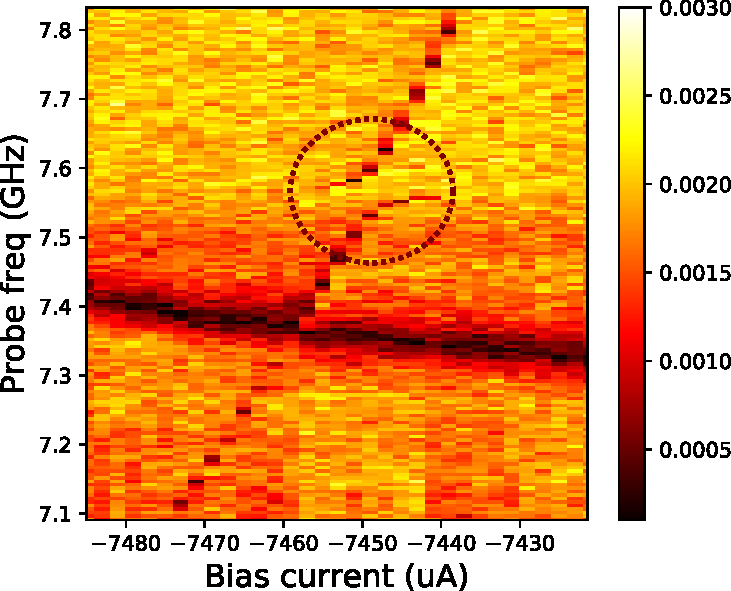
\includegraphics[width=0.7\textwidth]{STS_Anticross_ed.pdf} \hfill
	\caption[Взаимодействие кубита с резонансной двухуровневой системой]{Пример антикроссинга спектра кубита (узкая линия) с паразитной двухуровневой системой. Антикроссинг выделен кружком.} 
	\label{img: anticross}
\end{figure}

Интересно отметить, что на некоторых спектрах наблюдаются антипересечения линии кубита с некоторой резонансной системой, которые обусловлены когерентным взаимодействием с дефекными двухуровневыми системами, см. Рис.~\ref{img: anticross}. Как правило, эти системы расположены внутри слоя AlOx джозефсоновского контакта, и устранить их практически невозможно. Наличие дефектов в джозефсоновском переходе --- еще одна причина ограничения размеров джозефсоновского контакта: при большой площади переходов плотность дефектов становится достаточно значительной, что портит кубит и делает работу с ним невозможной. Именно поэтому необходимо изготавливать джозефсоновские переходы при помощи электронно-лучевой литографии, дающей разрешение примерно до 50 нм. 

Полученные в ходе однотоновой спектроскопии данные иллюстрируют стационарное рассеяние маломощного когеретного сигнала на кубите. Чтобы увидеть эффект насыщения, необходимо зафиксировать магнитное поле и измерить линию кубита в зависимости от амплитуды поля $\Omega$. Результаты данного измерения и их подгонка приведены на Рис.~ \ref{img: power_line}. 
\begin{figure}
	\centering
	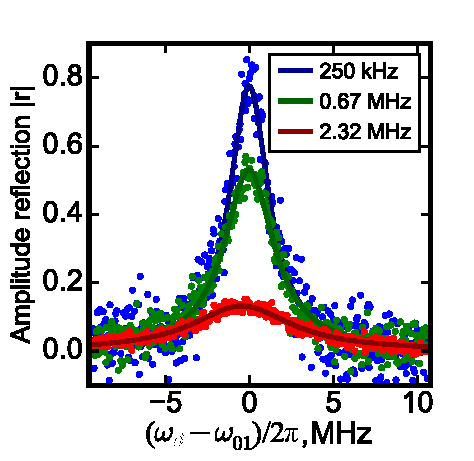
\includegraphics[width=0.6\textwidth]{Fig_2_PRA_phd.pdf} \hfill
	\caption[Насыщение резонансной флуоресценции на кубите]{Зависимость коэффициента отражения $r$ от амплитуды Раби $\Omega$, значения которой приведены на легенде. Линии подгонки получены при помощи формулы \eqref{eq: refl} для $\Gamma_1/2\pi = 2.2$~МГц, $\Gamma_2=\Gamma_1/2$.}
	\label{img: power_line}
\end{figure}
Подгоняя эти измерения при помощи аналитических выражений, можно определить $\Gamma_1$, $\Gamma_2$ и $\Omega$. Результаты подгонки однотоновой спектроскопии для нескольктх изучаемых кубитов приведены в Табл. \ldots.



Таким образом, в эксперименте мы показали, как кубит обнаруживает себя в спектроскопических измерениях, проводимых при помощи ВАЦ. Более того, результаты однотоновой спектроскопии уже позволяют определить ключевые параметры, описывающие стационарный режим резонансного рассеяния. Далее мы покажем, как состояние кубита эволюционирует во времени, проиллюстрируем динамику кубита и поля, излучаемого этим кубитом. 
\section{Неэластично рассеянное поле. Триплет Моллоу}
\label{sec: Triplet_meas}
Принципиальная особенность измерения, описанного нами как однотоновая спектроскопия, состоит в том, что измеряется излучение, рассеянное строго на частоте внешнего драйва $\omega_d$. Как подробно описано в разделе \ref{sec: scatt}, в стационарном режиме среднее состояние кубита не меняется со временем. Однако, ясно, что даже в этом случае кубит непрерывно взаимодействует с полем. Если мы измеряем энергию поля, то имеют место флуктуации поля, связанные с квантовыми скачками кубита из возбужденного в основное состояние и назад. Следствием этого является нетривиальный спектр рассеянного излучения, называемый также триплет Моллоу, см. \eqref{eq: mollow} и Рис.~\ref{fig: Mollow}. Подробно рассмотрев ранее теоретические особенности данного явления, покажем, каким образом триплет Моллоу можно получить в эксперименте.

Измерительная схема для наблюдения спектра неэластичного рассеяния достаточно тривиальна и отличается от однотоновой спектроскопии лишь тем, что вместо ВАЦ необходимо использовать СВЧ-генератор, а выходной сигнал измерять при помощи спектрального анализатора или высокоскоростного АЦП. Однако, непосредственно измерение спектра сопряжено с некоторыми практическими трудностями. Опишем их более подробно.

Для дальнейших рассуждений полезно оценить отношение сигнал-шум (ОСШ), с которым мы сталкиваемся при измерении рассеянного на кубите сигнала в интересующем нас режиме $\Omega \sim \Gamma_1$. Как и в большинстве электротехнических схем усиления, в нашей установке шум определяется первым каскадом усиления, и в схеме на Рис.~\ref{fig: schemes} это криогенный СВЧ-усилитель на базе транзистора с высокой подвижностью электронов, или HEMT-усилитель. В наших измерениях используются усилители от компании Low Noise Factory с эквивалентной шумовой температурой $T_n=3\text{-}5$~К. Достаточно хорошей оценкой для мощности рассеянного сигнала является величина $\hbar \omega_q\Gamma_1$, и если считать, что выбранная ширина полосы при измерениях выбирается порядка $\Gamma_1$, то для вычисления ОСШ нам достаточно сравнить $\omega_q$ и $T_n$. Несложно проверить что $T_n=1$~К соответствует частоте перехода $\omega_n/2\pi=20$~ГГц, поэтому для типичных частот кубитов от 4 до 8 ГГц ОСШ составляет примерно $0.05\text{-}0.1$. 

При рассмотренных ранее спектроскопических измерениях детектирование происходит в стационарном режиме, и поэтому есть возможность выбрать полосу частот входного фильтра составляет 10-100 Гц, что делает шум пренебрежимо малым по сравнению с сигналом. Однако, при измерении спектра мы имеем дело с флуктуациями поля, происходящими на временном масштабе порядка $T_1$, и поэтому полоса частот должна быть как минимум несколько МГц, и шум значительно превышает полезный сигнал. Дополнительно, необходимо избежать влияния $1/f$ шума, для чего измерение происходит при помеременном включении и выключении микроволнового сигнала (несколько десятков Гц), после чего одна частотная развертка вычитается из другой, и таким образом компенсируется низкочастотный шум. Результат измерений представлены на Рис.~\ref{fig: Mollow_w_fit}. Подгоняя полученный спектр, можно определить частоту Раби и константы $\Gamma_1$ и $\Gamma_2$ независимо от измерений среднего поля в стационарном состоянии, рассмотренных ранее. 
\begin{figure}
	\centering
	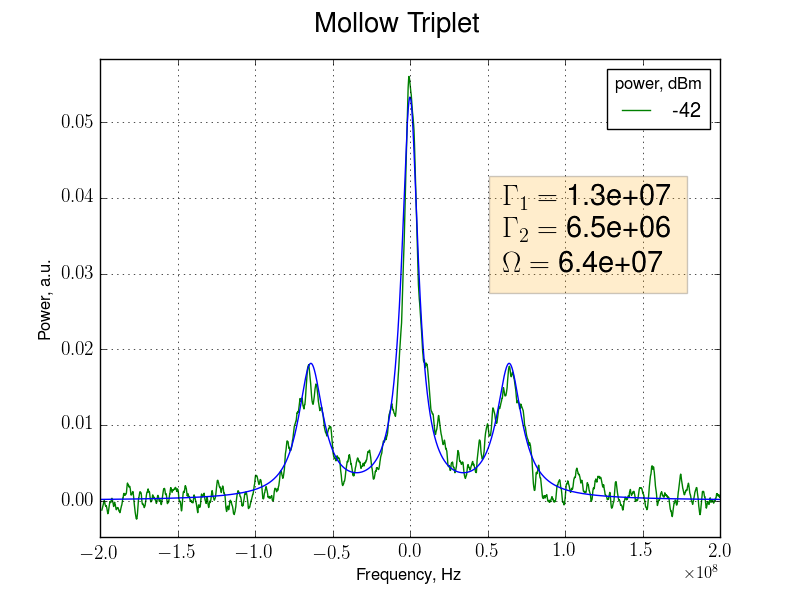
\includegraphics[width=1\textwidth]{Mollow Triplet_w_fit.png}
	\caption[Спектр неэластично рассеянного поля на кубите.]{Спектр неэластично рассеянного поля, полученный после $\sim 10^6$ усреднений единовременно измеренных спектров. Экспериментальная кривая дополнительно сглажена при помощи цифрового фильтра. Синяя линия представляет собой подгонку по формуле \eqref{eq: mollow}, параметры фита указаны на легенде.}
	\label{fig: Mollow_w_fit}
\end{figure}

Зависимость спектра флуоресценции от мощности поля, взаимодействующего с кубитом, представлена на Рис.~\ref{fig: Mollow_w_fit}. Удаление боковых пиков от центрального максимума связано с увеличением $\Omega$. Отметим также, что с увеличением $\Omega$ растет относительная доля энергии, приходящаяся на неэластичное рассеяние. Этот неочевидный результат можно качественно обосновать следующим образом. При $\Omega \gg \Gamma_1$ средняя заселенность кубита практически равна 0.5, а поэтому в среднем кубит излучает б\'{o}ольшую мощность $P \sim \braket{\sz}$. В свою очередь, мощность эластично рассеянного сигнала пропорциональна $|r\Omega|^2$, где $r$ определяется выражением \eqref{eq: refl} и убывает как $1/\Omega^2$. Таким образом, эластично рассеянная мощность убывает, а неэластично рассеянная мощность --- возрастает. 

\begin{figure}[h]
	\centering
	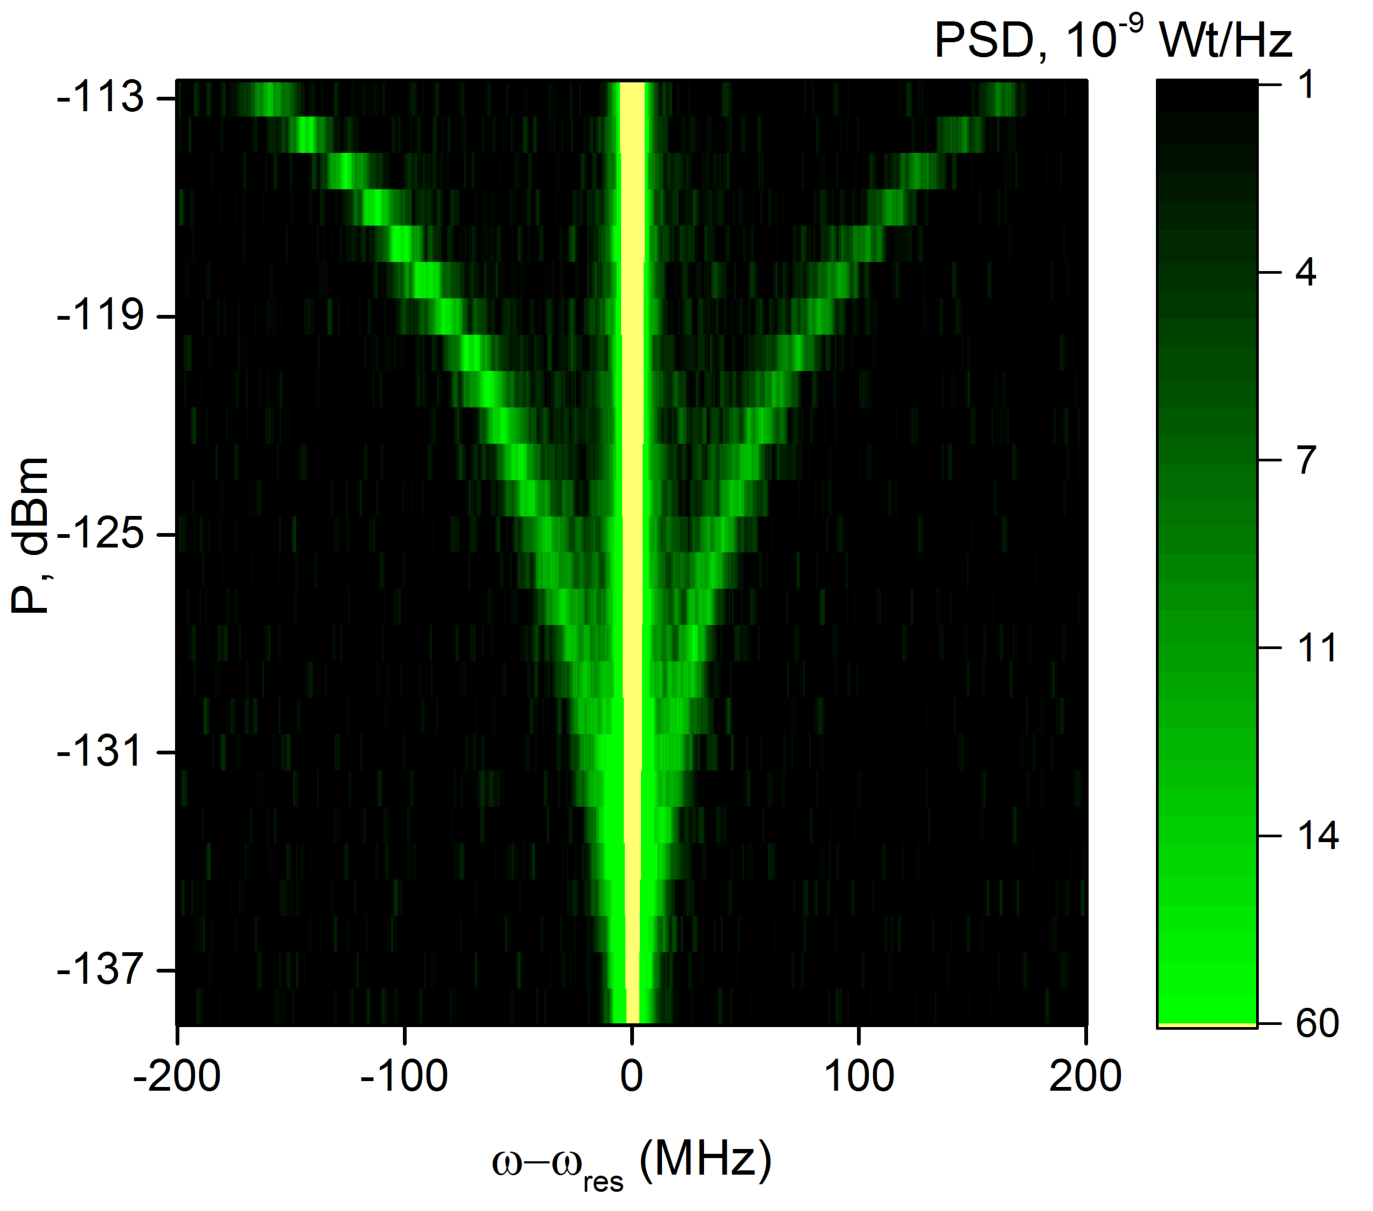
\includegraphics[width=0.7\textwidth]{Mollow_power.pdf}
	\caption[Зависимость триплета Моллоу от мощности драйва.]{Зависимость спектра неэластичного рассеяния от мощности сигнала, взаимодействующего с кубитом. }
	\label{fig: Mollow_w_fit}
\end{figure} 
Мы рассмотрели измерения резонансной флуоресценции кубита в стационарном состоянии, показав эластично рассеянное поле, измеряемое при помощи ВАЦ, и неэластично рассеянное поле, измеряемое с помощью СА. Однако, методы микроволновых измерений позволяют непосредственно изучать динамику кубита под воздействием коротких импульсов поля. Импульсным измерениям кубитов посвящена следующая глава данной диссертационной работы. 
\section{Временная динамика состояния кубита}
%рассказ об импульсных схемах и несколько картинок Раби (мб с фитом)
После подробного изучения стационарного рассеяния на кубите интересным представляется показать временную динамику состояния кубита под действием кратковременных импульсов, длительность которых значительно меньше времени жизни кубитов, несущая частота близка к резонансу, а Раби частота значительно больше чем $\Gamma_1$. Схема для формирования импульсов представлена на Рис.~\ref{fig: pulse_setup_1}. В ее основе лежит принцип гетеродина. Во входной части схемы  формирование возбуждающих кубит импульсов происходит за счет квадратурного СВЧ-смесителя, подключенного на повышение частоты. Короткие импульсы на выходе миксера R образуются после смешивания непрерывной волны на несущей частоте $\omega_{LO}$ (обозначается как LO от англ. \textit{Local Oscillator}), подаваемой на вход смесителя L и коротких импульсов на промежуточной частоте $\omega_{IF}$, подаваемых на вход I. Несущая частота непрерывного сигнала находится в гигагерцовом диапазоне и производится при помощи СВЧ-генератора.  

\begin{figure}[h]
	\centering
	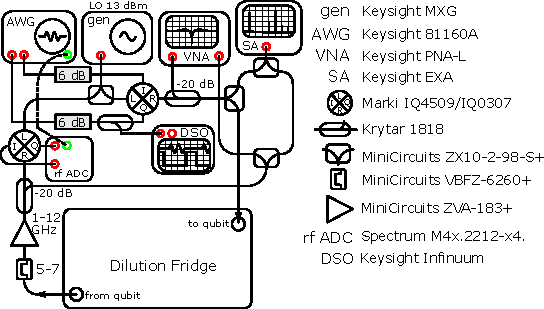
\includegraphics[width=0.98\textwidth]{pulse_setup_1.pdf}
	\caption[Схема для изучения динамики кубита под воздействием коротких импульсов]{Принципиальная схема подключения СВЧ-электроники для изучения динамики кубита под воздействием импульсов. На легенде приведены используемые модели приборов и других компонентов схемы. Красные окружности символизируют сигнальные входы/выходы приборов, зеленые окружности --- входы/выходы триггера для синхронизации оцифровщика с ГИПФ. Черные линии символизируют коаксиальные провода, в местах пересечений проводов на схеме контакт между ними отсутствует. }
	\label{fig: pulse_setup_1}
\end{figure} 
Импульсы промежуточной частоты создаются при помощи генераторов сигналов произвольной формы (сокращенно ГИПФ или AWG). Частоты подбираются таким образом, чтобы одна из ближайших к LO смешанных компонент, называемых также сайдбендами (от англ.~\textit{sidebands}), сравнивалась с частотой кубита: $\omega_q = \omega_{LO} \pm \omega_{IF}$. Короткие импульсы имеют длительность примерно 2-100 нс и несущую частоту ПЧ от 10 до 100 МГц. При этом, смеситель дает большое количество других гармоник вида $\omega_{LO} \pm n\omega_{IF}$, которые при достаточной интенсивности могут искажать динамику кубита. По этой причине необходимо точно калибровать мощность резонансного сайдбенда и как можно лучше подавлять остальные сайдбенды. Это делается при помощи калибровки квадратурных смесителей, состоящей в подборе смещений нулевого уровня, относительной фазы и амплитуды импульсов, подаваемых с AWG на входы I и Q смесителя. Более подробно о калибровке миксеров можно прочитать в работах \cite{Schneider2015, jeffrey2014fast}.

Выходная часть схемы служит для анализа прошедшего через кубит (рассеянного на кубите) сигнала и может быть реализована несколькими способами. На Рис.~\ref{fig: pulse_setup_1} приведен наиболее правильный вариант, когда вышедший из криостата сигнал подается на вход R выходного смесителя и  претерпевает преобразование частоты вниз. На выходной смеситель подается тот же сигнал LO, который использовался на повышающем миксере, а выходы I и Q содержат сигнал на промежуточной частоте, который несет с точностью до константы ту же фазу, что и высокочастотный рассеянный сигнал. Эта схема позволяет полностью восстановить временную развертку рассеянного поля, но для ее реализации требуется наладка работы высокоскоростного АЦП и его качественная (с точностью лучше чем 1 нс) синхронизация с ГИПФ, что сопряжено с определенными техническими сложностями. Поэтому при изучении рассеянного поля применялись также более простое решение --- работа в режиме $\omega_{IF}=0$ без повышения и понижения частоты и оцифровка сигнала непосредственно при помощи ВАЦ. Вне зависимости от использования промежуточной частоты, рассеянный сигнал можно анализировать на СА, который также используется при калибровке миксеров. 

\subsection{Раби-осцилляции}
После сборки и настройки схемы изучаются Раби осцилляции кубита под действием импульса. Наиболее простой вариант измерений Раби осцилляций может быть реализован при измерениях на векторном анализаторе без применения промежуточной частоты. При этом на входы I и Q входного миксера подаются импульсы постоянного тока, длительность которой сответствует длительности эволюции кубита, а промежуток между ними должен многократно превышать время жизни кубита, чтобы за время отсутствия драйва кубит успевал отрелаксировать в основное состояние. Эти импульсы модулируют несущую волну на входе L, частота которой совпадает при этом с частотой кубита. Выходной миксер используется в аналогичном режиме в качестве <<чоппера>>: на вход L подается провзаимодействовавший с кубитом сигнал, а на входы I и Q подаются импульсы постоянного напряжения. Их задержка подобрана таким образом, чтоб начало импульсов совпадало по времени с концом импульсного сигнала, прошедшего через кубит. При этом из рассеянного сигнала вырезается начальный импульс, а то поле, которое излучается после импульса, зависит только от состояния кубита на момент конца Раби-эволюции. Блок-схема вышеописанного эксперимента представлена на Рис.~\ldots.

\begin{figure}[h]
	\centering
	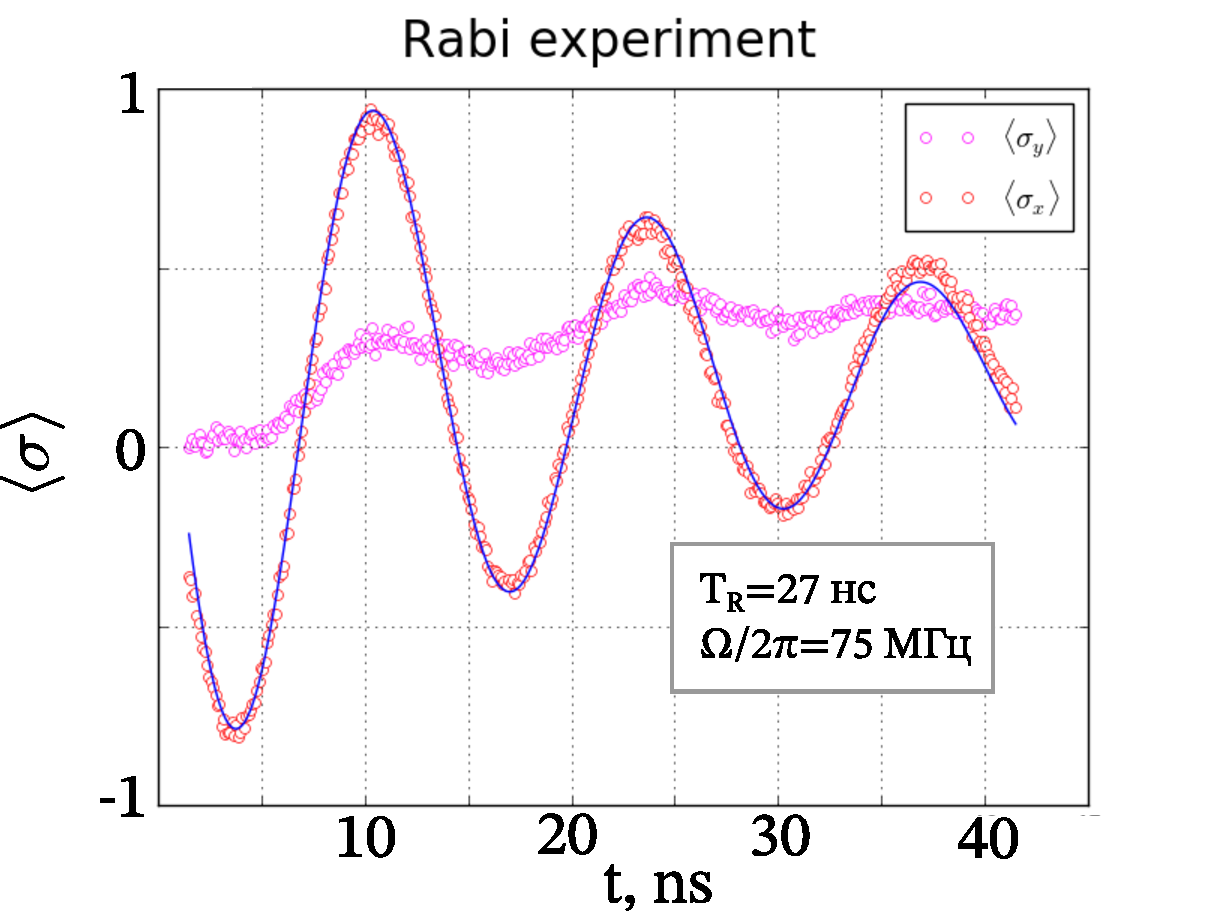
\includegraphics[width=0.7\textwidth]{Rabi.pdf}
	\caption[Раби осцилляции кубита в линии, полученные при измерении рассеянного поля]{Осцилляции Раби: квадратуры оцифрованного ВАЦ напряжения в зависимости от длительности управляющего импульса. Подгонка при помощи экспоненциально затухающей гармонической функции дает характерное время затухания $T_R$ и частоту осцилляций $\Omega$.}
	\label{fig: rabi_ocs}
\end{figure} 

Результат измерения ВАЦ в зависимости от длительности возбуждающего импульса представлен на Рис.~\ref{fig: rabi_ocs}. Поскольку фаза переизлучаемого кубитом поля совпадает с фазой состояния кубита, то после вычета задержки распространения сигнала осцилляции ярко выражены в действительной части. Ненулевая мнимая часть является проявлением наличия некоторого паразитного сигнала, проходящего через линию,  и, по всей вероятности, связанного с объемными модами держателя образцов.  
\begin{figure}[h]
	\centering
	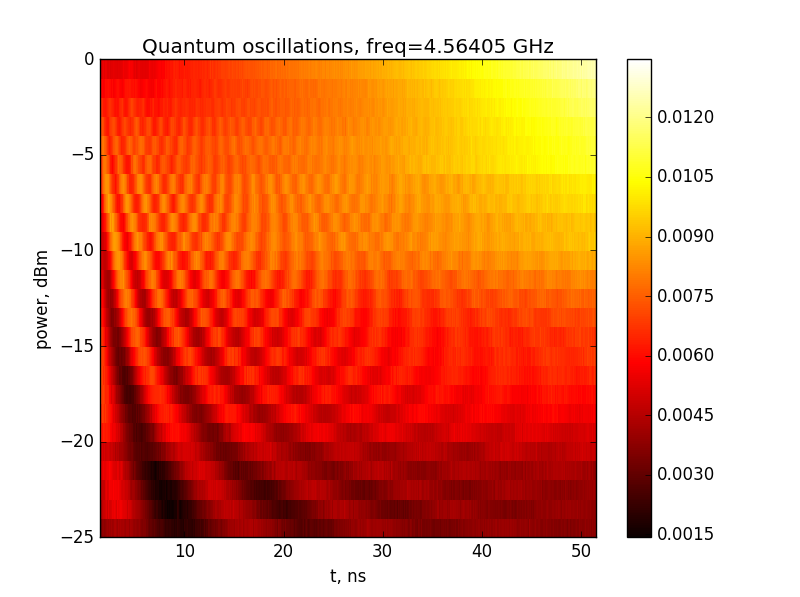
\includegraphics[width=0.95\textwidth]{SPS_oscillations_3D_2}
	\caption[Зависимость Раби осцилляций от мощности сигнала]{Осцилляции Раби при различной мощности управляющего сигнала. Общий фон меняется при увеличении мощности из-за паразитного сигнала на частоте LO, которого практически невозможно избежать в схеме с нулевой промежуточной частотой}
	\label{fig: rabi_ocs}
\end{figure} 
Характерная отличительная особенность осцилляций Раби --- линейная пропорциональность Раби частоты и амплитуды возбуждающего сигнала. Для выявления этой пропорциональности осцилляции измеряются в широком диапазоне амплитуд входного сигнала, см. Рис.~\ref{fig: rabi_ocs}. Из осцилляций, измеренных при различных значениях амплитуды, определяется зависимость $\Omega(\sqrt{P})$, которая хорошо аппроксимируется линейной зависимостью, см. Рис.\ref{img: Rabi_from_amp_2},
\begin{figure}[h]
	\centering
	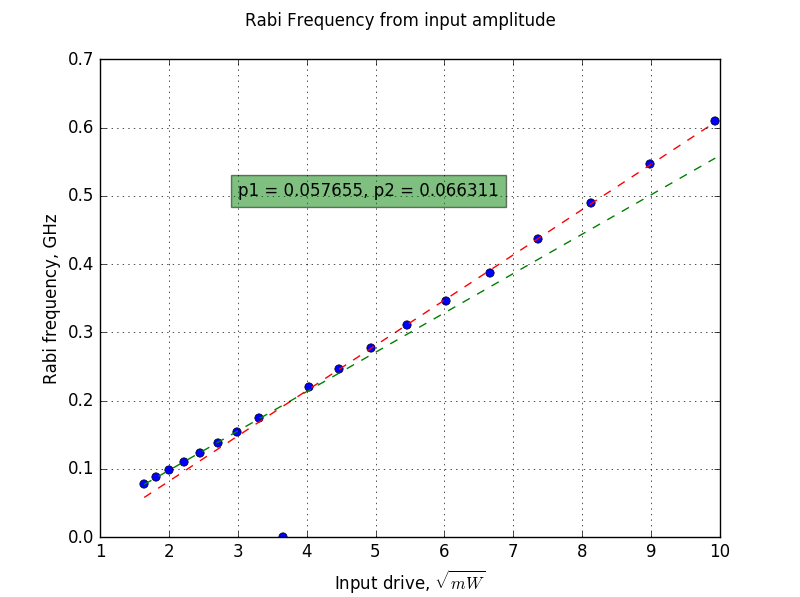
\includegraphics[width=0.9\linewidth]{Rabi_freq_from_input_amplitude} 
	\caption[Зависимость Раби частоты от амплитуды входного поля.]{Зависимость Раби частоты от амплитуды входного поля, построенная на основе данных  Рис.~\ref{fig: rabi_ocs}. Результаты хорошо аппроксимируются линейной зависимостью, однако можно заметить что начальный участок, соответствующий малой амплитуде, отличается коэффициентом пропорциональности (зеленая пунктирная линия) от остальной части (красная пунктирная линия). Это может быть связано с нелинейностью смесителей или несовершенством внутренних аттенюаторов ВАЦ.}
	\label{img: Rabi_from_amp_2}  
\end{figure}
что еще раз подтверждает квантовую природу наблюдаемых осцилляций. Нужно отметить, что наблюдаемой величиной здесь является $\braket{\hat{\sigma}_x}$ или $\braket{\hat{\sigma}_y}$ (в зависимости от измеряемой квадратуры). Поэтому фаза наблюдаемых осцилляций Раби сдвинута на $\pi/2$ относительно осцилляций в более типичного случае, когда измеряется средняя населенность кубита $\braket{\hat{\sigma}_z}$, например, при помощи резонатора, связанного с кубитом. 

\subsection{Импульсное определение дефазировки}
Помимо рассмотренных в предыдущем разделе осцилляций Раби, импульсные измерения позволяют независимо определить полную дефазировку кубита $\Gamma_2$. Для этого достаточно приложить импульс, поворачивающий кубит на угол $\pi/2$. Откалибровать длительность такого импульса можно по осцилляциям Раби, а именно, нужно определить при какой длительности импульса переизлученное поле кубита оказывается максимальным. Прикладывая к кубиту $\pi/2$-импульс и меняя задержку между концом этого импульса и считывающим импульсом, мы визуализируем затухание когерентности в кубите, см. Рис.~\ref{fig: G2}. Экспоненциальная подгонка полученного сигнала дает численное значение $\Gamma_2$. 

\begin{figure}[h]
\centering
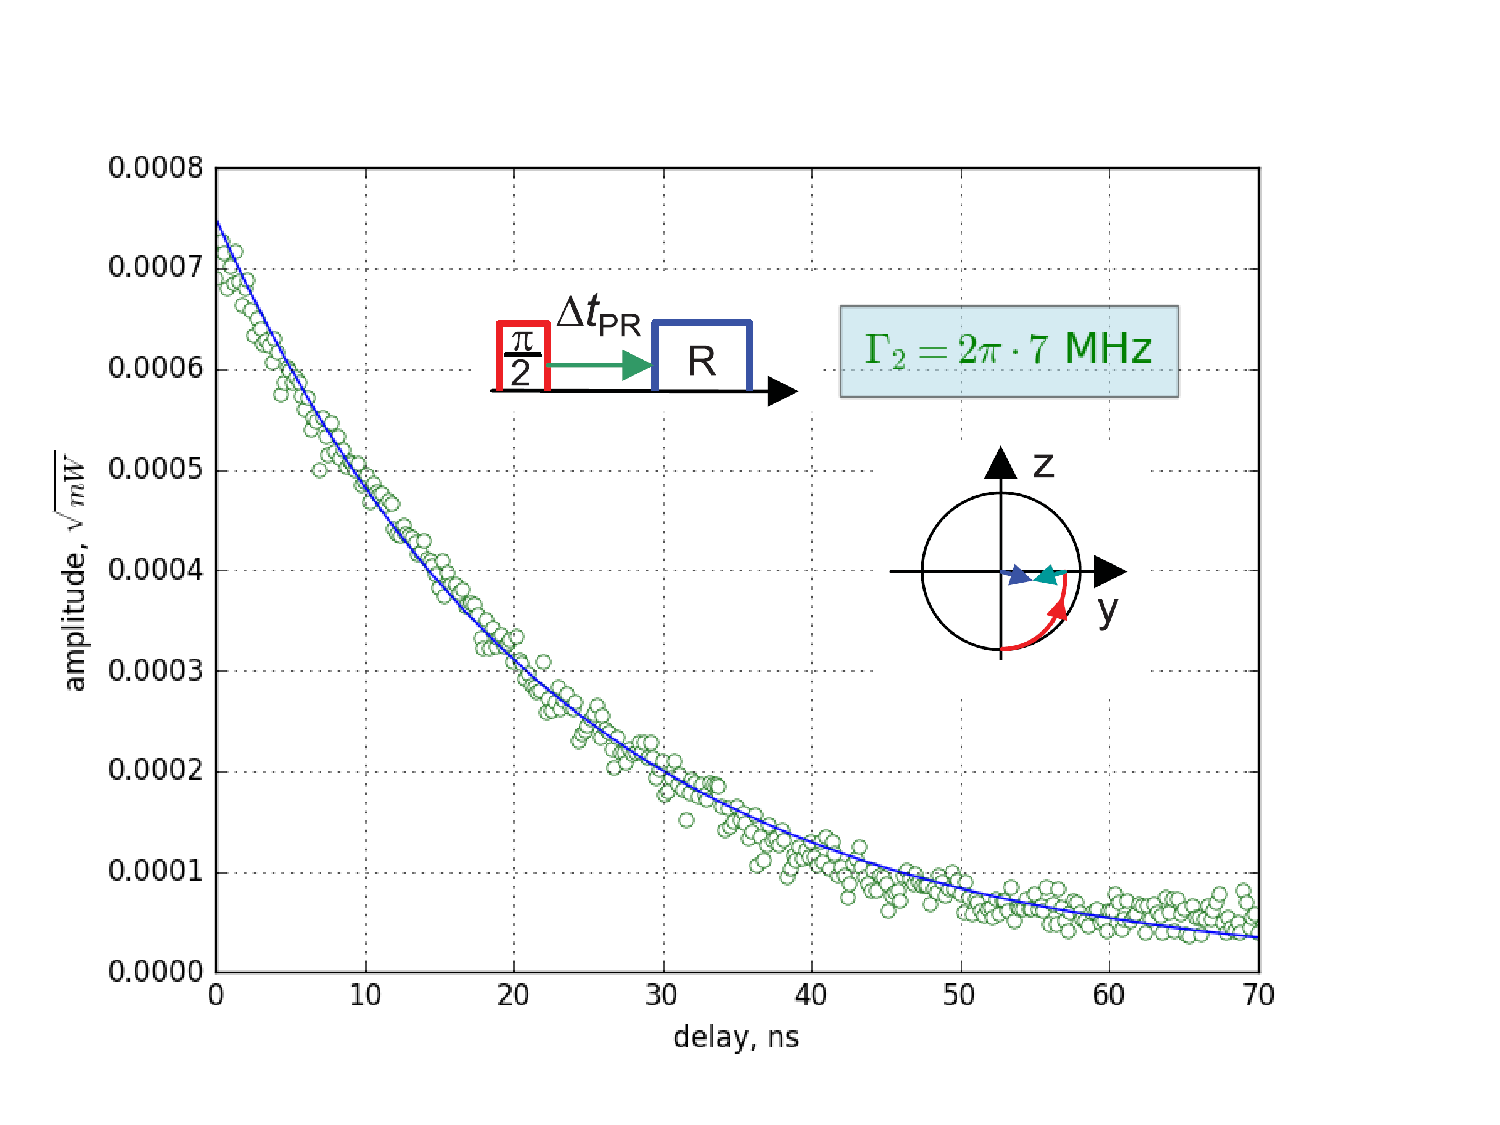
\includegraphics[width=0.95\textwidth]{G2}
\caption[Измерение полной дефизировки при помощи $\pi/2$-импульса.]{Измерение полной дефизировки при помощи $\pi/2$-импульса. На вставке приведена схема импульсов и динамика кубита на сфере Блоха. Полученное значение $\Gamma_2/2\pi=7$ МГц хорошо соотвествует величине релаксации $\Gamma_1=13$~МГц, определенной из стационарного рассеяния в той же рабочей точке по потоку для исследуемого кубита.}
\label{fig: G2}
\end{figure}

После описания импульсных измерений мы переходим к рассмотрению кубита как одноатомной нелинейной среды и покажем, почему одиночный кубит в линии является хорошей платформой для изучения нелинейных квантовых эффектов.
\section{Кубит в качестве нелинейной среды}
После того, как промерена однотоновая спектроскопия кубита и измерена его эволюция под действием внешнего поля, необходимо убедиться в нелинейном поведении кубита в линии. В некотором смысле, все предыдущие результаты показывают, что мы действительно имеем дело с двухуровневой системой, которая по своей сути уже является сильно нелинейным объектом. Тем не менее, мы считаем нужным провести параллели с оптикой на естественных атомах в видимом диапазоне света. В традиционной оптике используется понятие \textit{нелинейной среды}, в которой нарушается пропорциональность электрического поля и поляризации. При распространении света в некотором веществе быстро осциллирующее электрическое поле волны $\tilde{E}(t)$ поляризует атомы или молекулы этого вещества. Поляризация среды может быть представлена в виде:
%\begin{figure}[ht]
%	\centering
%		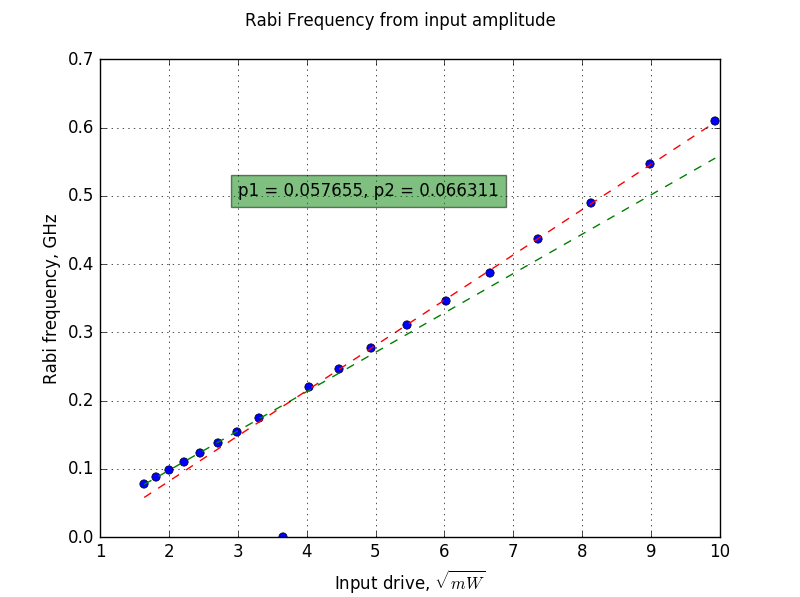
\includegraphics[width=1\linewidth]{Rabi_freq_from_input_amplitude}
%	\caption[Зависимость Раби частоты от амплитуды входного поля.]{Зависимость Раби частоты от амплитуды входного поля, построенная на основе данных  Рис.~\ref{fig: rabi_ocs}}
%	\label{img: Rabi_from_amp_2} 
%	\hfill
%\end{figure}
\begin{equation}
\tilde{P}(t) = \epsilon_0\left(\chi^{(1)}\tilde{E}(t) + \chi^{(2)}\tilde{E}^2(t) + \chi^{(3)}\tilde{E}^3(t) + \ldots\right)
\label{eq: nonlin_susc}
\end{equation}
Коэффициенты $\chi^{(2)}$ и $\chi^{(3)}$ называются нелинейной восприимчивостью. Разложение \eqref{eq: nonlin_susc} применимо в том случае, когда излучение нерезонансно, то есть его частота не совпадает с частотами атомных или молекулярных переходов. Это условие не выполняется при облучении кубита на резонансной частоте, но тем не менее, на основе разложения восприимчивости по степеням поля мы можем сделать некоторые полезные выводы. В случае одиночного искусственного атома мы имеем дело с насыщаемым рассеивателем --- двухуровневой системой, которая поляризуется под воздействием внешней волны. Значение поляризации атома можно получить как среднее значение дипольного момента, взятое по стационарному состоянию:
\begin{equation}
\tilde{P}(t) = \tr(\hat{\mu}\hat{\rho}_{st}) = \mu_{01}\rho_{10} + \mu_{10}\rho_{01}.
\end{equation}

Пользуясь \eqref{eq: stat_sol} и определяя восприимчивость из соотношения $\tilde{P} = \chi\tilde{E}$, получаем:
\begin{equation}
\chi = \frac{|\mu|^2}{\epsilon_0\hbar\Gamma_2}\frac{i-\delta\omega/\Gamma_2}{1+(\delta\omega/\Gamma_2)^2 + \Omega^2/\Gamma_1\Gamma_2},
\end{equation}
см. также \cite{boyd2003nonlinear}. Как мы отмечали ранее, выражение $\Omega^2/\Gamma_1\Gamma_2$ характеризует степень насыщенности двухуровневой системы и может быть обозначено как ${E^2}/{E^2_s}$, где $E_s$ --- напряженность насыщения, которую также можно выразить в виде частоты Раби $\Omega_s$: 
\begin{equation}
E_s^2 = \frac{\hbar^2\Gamma_1\Gamma_2}{4|\mu|^2}, \quad \Omega_s = \sqrt{\Gamma_1\Gamma_2}/2.
\label{eq: E_s}
\end{equation}
В общем случае, выражение $\Omega^2/\Gamma_1\Gamma_2$ не является малым и поэтому использовать разложение \eqref{eq: nonlin_susc} по степеням $\Omega \sim E$ в явном виде нельзя. Тем не менее, мы можем написать первые члены этого разложения:  
\begin{equation}
\chi\approx\frac{|\mu|^2}{\epsilon_0\hbar\Gamma_2}\frac{i-\delta\omega/\Gamma_2}{1+(\delta\omega/\Gamma_2)^2}\left[1-\frac{1}{1+(\delta\omega/\Gamma_2)^2}\frac{E^2}{E^2_s}\right].
\label{eq: chi}
\end{equation}
Можно отметить, что слагаемое, пропорциональное $E^2$, характерно для нелинейной восприимчивости $\chi^{(3)}$, тогда как $\chi^{(2)}=0$ для кубита. Это согласуется с общим свойством нелинейных центросимметричных сред, в которых возникает нелинейность третьего и более высоких порядков, но отсутствует нелинейность второго порядка. 
Концептуально близкое к задаче рассеяния волны на кубите явление из нелинейной оптики --- зависящий от мощности показатель преломления среды, или т.н. оптический эффект Керра. Известно, что при эффекте Керра возникающая нелинейная поляризация среды может быть записана в виде:
\begin{equation}
\tilde{P}^{N\!L} = \chi \tilde{E} = \left(\chi^{(1)} + 3\chi^{(3)}\tilde{E}^2\right)\tilde{E}.
\label{eq: P_NL}
\end{equation}
Сопоставляя \eqref{eq: P_NL} и \eqref{eq: chi}, получаем выражение для $\chi^{(3)}$:
\begin{equation}
\chi^{(3)} = -\frac{|\mu|^2}{3\epsilon_0\hbar\Gamma_2}\left[\frac{\delta\omega/\Gamma_2-i}{1+(\delta\omega^2/\Gamma^2_2)^2}\frac{1}{E^2_s}\right] = \frac{4}{3}\frac{|\mu|^4}{\epsilon_0\hbar^3\Gamma_1\Gamma_2^2}\frac{i-\delta\omega/\Gamma_2}{(1+\delta\omega^2/\Gamma_2^2)^2}.
\label{eq: chi_3}
\end{equation}
Полученный результат можно использовать для сравнения величины нелинейности, возникающей на кубите, с типичными значениями $\chi_{(3)}$ в задачах традиционной видимой оптики. Для наблюдения резонансной флуоресценции в видимом диапазоне свет может рассеивается, к примеру, на разреженном газе из атомов натрия. Таблица \ref{Tab2} иллюстрирует основные экспериментальные параметры, определяющие нелинейность, и конечные значения нелинейной восприимчивости. 
\begin{table} [htbp]
	\centering
	\changecaptionwidth\captionwidth{15cm}
	\caption{Экспериментальные характеристики нелинейных квантовооптических систем в открытом пространстве}\label{Tab2}%
	\begin{tabular}{| p{2.4cm} | p{3.2cm} | p{3.2cm}l |}
		\hline
		\hline
		Параметр   & \centering Кубит в линии & \centering Пары натрия \cite{boyd2003nonlinear} & \\
		\hline
		$N$ &\centering  $1$  &\centering $10^{14}$ & \\
		$\mu$, Кл$\cdot$м &\centering  $\sim 10^{-24}$   &\centering  $\sim10^{-29}$ &\\
		$\delta\omega$, Гц &\centering  $\sim 0$  &\centering $\sim10^{10}$ &\\
		$\Gamma_1$, Гц &\centering  $\sim10^6$  &\centering $\sim10^8$ & \\
		$\Gamma_2$ &\centering  $\Gamma_1/2$  &\centering $\Gamma_1/2$ & \\
		$\chi^{(3)}$, \text{м}$^2$/\text{В}$^2$ &\centering $\sim i\cdot 10^{-15}$   &\centering  $\sim 10^{-16}$ & \\
		\hline
		\hline
	\end{tabular}
\end{table}

Отметим ряд принципиальных различий между рассеянием микроволн на одиночном кубите и рассеянии видимого света на облаке атомов. Во-первых, имеется принципиальная возможность изучать рассеяние при нулевой отстройке $\delta\omega\!=\!0$. В случае облака атомов, на резонансной частоте перехода происходит сильное многократное поглощение (и переизлучение) света во всех направлениях, и задетектировать их чрезвычайно сложно. В свою очередь, одиночный кубит излучает поле в копланарный волновод, это поле усиливается криогенным усилителем и измеряется при помощи АЦП. С учетом небольших потерь в коаксиальных проводах и аттенюаторов на 0 дБ, через которые сигнал с кубита проходит перед попаданием на усилитель, схема позволяет измерить до 99\% сигнала, рассеянного кубитом, что проявляется в экспериментах по генерации одиночных фотонов \cite{ZhouHighEfficiency}. Во-вторых, среднее значение $\chi^{(3)}$ на одном искусственном атоме сравнимо и даже превышает аналогичную величину для паров натрия, где в облаке находится макроскопическое количество атомов. Изложим некоторые рассуждения, которые помогут понять необычность обсуждаемого экспериментального режима. Из \eqref{eq: E_s} очевидно, что Раби частота насыщения практически равна $\Gamma_1$, что эквивалентно означает большую чувствительность (и даже нелинейность кубита) кубита к полям на уровне одиночных фотонов. Поэтому можно ожидать, что типичные нелинейнооптические эффекты, как например, волновое смешение, будут проявляться при рассеянии на атоме совершенно необычным образом.

Суммируя вышеизложенное, нелинейность на одном искусственном атоме по порядку величины практически сравнивается с нелинейностью макроскопического количества атомов в нелинейной среде. Это дает возможность изучать необычные квантовые эффекты в рамках нелинейной оптики, о которых пойдет речь в следующих главах данной диссертационной работы.  В следующем подразделе мы кратко опишем основные принципы волнового смешения и изложим результаты смешения двух резонансных сигналов на одиночном искусственном атоме в непрерывном режиме.




